\documentclass[12pt,a4paper]{article}

% ── Fonts and Encoding
\usepackage[T1]{fontenc}
\usepackage{mathptmx}
\usepackage[utf8]{inputenc}

% ── Page Layout
\usepackage[top=1in, bottom=1in, left=1.25in, right=1.25in]{geometry}
\usepackage{setspace}
\onehalfspacing

% ── Math
\usepackage{amsmath, amssymb}

% ── Tables and Figures
\usepackage{booktabs}
\usepackage{tabularx}
\usepackage{array}
\usepackage{float}
\usepackage{graphicx}
\usepackage[font=small, labelfont=bf]{caption}

% ── Misc
\usepackage{enumitem}
\usepackage[hidelinks]{hyperref}
\usepackage{fancyhdr}
\usepackage{titlesec}

% ── Prevent overflow
\usepackage{microtype}
\tolerance=1000
\emergencystretch=3em
\setlength{\parindent}{0pt}
\setlength{\parskip}{6pt}

% ── No header or footer line, just page number
\pagestyle{fancy}
\fancyhf{}
\fancyfoot[C]{\thepage}
\renewcommand{\headrulewidth}{0pt}

% ── Section formatting (clean, numbered, not all-caps)
\titleformat{\section}[block]{\large\bfseries}{\thesection.}{0.5em}{}
\titleformat{\subsection}[block]{\normalsize\bfseries}{\thesubsection}{0.5em}{}
\titleformat{\subsubsection}[block]{\normalsize\itshape}{\thesubsubsection}{0.5em}{}
\titlespacing*{\section}{0pt}{18pt}{8pt}
\titlespacing*{\subsection}{0pt}{12pt}{4pt}

% ── Table column types
\newcolumntype{L}[1]{>{\raggedright\arraybackslash}p{#1}}
\newcolumntype{R}[1]{>{\raggedleft\arraybackslash}p{#1}}

\begin{document}

% ── Title Page
\begin{titlepage}
\centering
\vspace*{2cm}

{\Large \textbf{JAWAHARLAL NEHRU UNIVERSITY}}\\[0.3cm]
{\large Centre for Economic Studies and Planning}\\[0.3cm]
{\large School of Social Sciences}\\[2.5cm]

{\LARGE \textbf{Dissertation Progress Report}}\\[0.4cm]
{\Large \textit{ARDL Modelling and Empirical Results}}\\[1.8cm]

{\Large \textbf{Asymmetric Pass-Through of Global Brent Crude Oil\\[0.2cm]
Shocks to India's Monthly CPI Inflation (2004--2024):}\\[0.2cm]
\textit{Evidence from an Asymmetric ADL Framework}}\\[2.5cm]

\begin{tabular}{rl}
\textbf{Student:}    & Aniket Pandey \\[0.3cm]
\textbf{Supervisor:} & Prof. Shakti Kumar \\[0.3cm]
\textbf{Programme:}  & MS Economics, 2026 \\[0.3cm]
\textbf{Date:}       & April 2026 \\
\end{tabular}

\vfill
\end{titlepage}

\newpage
\tableofcontents
\newpage


% ═══════════════════════════════════════════════════
\section{Overview}
% ═══════════════════════════════════════════════════

This report covers the modelling work done so far for the dissertation. The question we are trying to answer is simple: when global oil prices go up, does India's consumer inflation go up more than it comes down when oil prices fall?

India imports around 85 per cent of its crude oil. So oil price changes feed into transport costs, fuel prices, and eventually into consumer prices. But the pass-through might not be symmetric. Prices might go up quickly when oil rises (the ``rockets'' part) and come down slowly, or not at all, when oil falls (the ``feathers'' part). This is what the literature calls ``rockets and feathers.''

The model uses monthly data from April 2004 to December 2024 (249 observations). The main tool is an asymmetric Autoregressive Distributed Lag (ADL) model, where positive and negative oil price changes enter as separate variables. All inference uses Newey-West standard errors to handle heteroskedasticity.

The entire analysis runs from a single R script (\texttt{analysis.R}) and produces all the tables and figures automatically.


% ═══════════════════════════════════════════════════
\section{Data}
% ═══════════════════════════════════════════════════

\subsection{Sources}

Four monthly series are used. Table~\ref{tab:datasources} lists them.

\begin{table}[H]
\centering
\caption{Data sources}
\label{tab:datasources}
\small
\begin{tabularx}{\textwidth}{L{2.5cm} L{4.5cm} L{3cm} L{3cm}}
\toprule
\textbf{Variable} & \textbf{Description} & \textbf{Source} & \textbf{Coverage} \\
\midrule
CPI        & Consumer Price Index, All Items (2015=100) & OECD via FRED       & Apr 2004 -- Dec 2024 \\
Brent      & Brent crude oil (USD/barrel)               & IMF via FRED        & Apr 2004 -- Dec 2024 \\
INR/USD    & Exchange rate (monthly avg.)                & Fed via FRED        & Apr 2004 -- Dec 2024 \\
IIP        & Index of Industrial Production              & RBI DBIE            & Apr 2004 -- Dec 2024 \\
\bottomrule
\end{tabularx}
\end{table}

The IIP series needed chain-linking because RBI publishes it in two base years (2004--05 and 2011--12). The two series overlap from April 2012 to January 2017, and the overlap-ratio method gives a splice factor of about 0.627. A Python script handles this, and the chained series has no visible jump at the splice point.

After merging and trimming to the study window, we get 249 monthly observations with no missing values.

\subsection{Descriptive statistics}

Table~\ref{tab:descstats} shows the summary statistics.

\begin{table}[H]
\centering
\caption{Descriptive statistics (April 2004 to December 2024)}
\label{tab:descstats}
\small
\begin{tabular}{lrrrrr}
\toprule
\textbf{Variable} & \textbf{N} & \textbf{Mean} & \textbf{Std.\ Dev.} & \textbf{Min} & \textbf{Max} \\
\midrule
CPI Index                        & 249 & 93.97  & 35.71  & 41.79   & 159.20 \\
Brent (USD)                      & 249 & 75.08  & 24.26  & 26.85   & 133.59 \\
INR/USD                          & 249 & 60.21  & 13.89  & 39.27   & 84.97  \\
IIP Index                        & 249 & 109.97 & 24.46  & 54.00   & 160.00 \\
Oil INR                          & 249 & 4490.59& 1692.95& 1464.13 & 9190.63\\
\midrule
$\Delta\ln\text{CPI}$ (\%)      & 248 & 0.54  & 0.75  & $-$1.66 & 4.47 \\
$\Delta\ln\text{Oil}$ (\%)      & 248 & 0.58  & 8.89  & $-$45.37& 23.20\\
$\Delta\ln\text{EXR}$ (\%)      & 248 & 0.27  & 1.67  & $-$4.14 & 6.56 \\
$\Delta\ln\text{IIP}$ (\%)      & 248 & 0.37  & 8.28  & $-$77.49& 51.30\\
$\Delta\text{Oil}^{+}$ (\%)     & 248 & 3.60  & 4.58  & 0.00    & 23.20\\
$\Delta\text{Oil}^{-}$ (\%)     & 248 & $-$3.02& 6.02  & $-$45.37& 0.00 \\
\bottomrule
\end{tabular}
\end{table}

Monthly CPI inflation averages about 0.54\%, which is roughly 6.5\% per year. Oil prices in rupee terms are far more volatile than CPI (standard deviation of 8.89\% versus 0.75\%). The positive oil changes average 3.60\% while the negative changes average $-$3.02\%, so the drops are less frequent but larger in magnitude.

Figure~\ref{fig:rawseries} shows the raw level series, and Figure~\ref{fig:logdiff} shows the log-differenced (stationary) versions.

\begin{figure}[H]
\centering
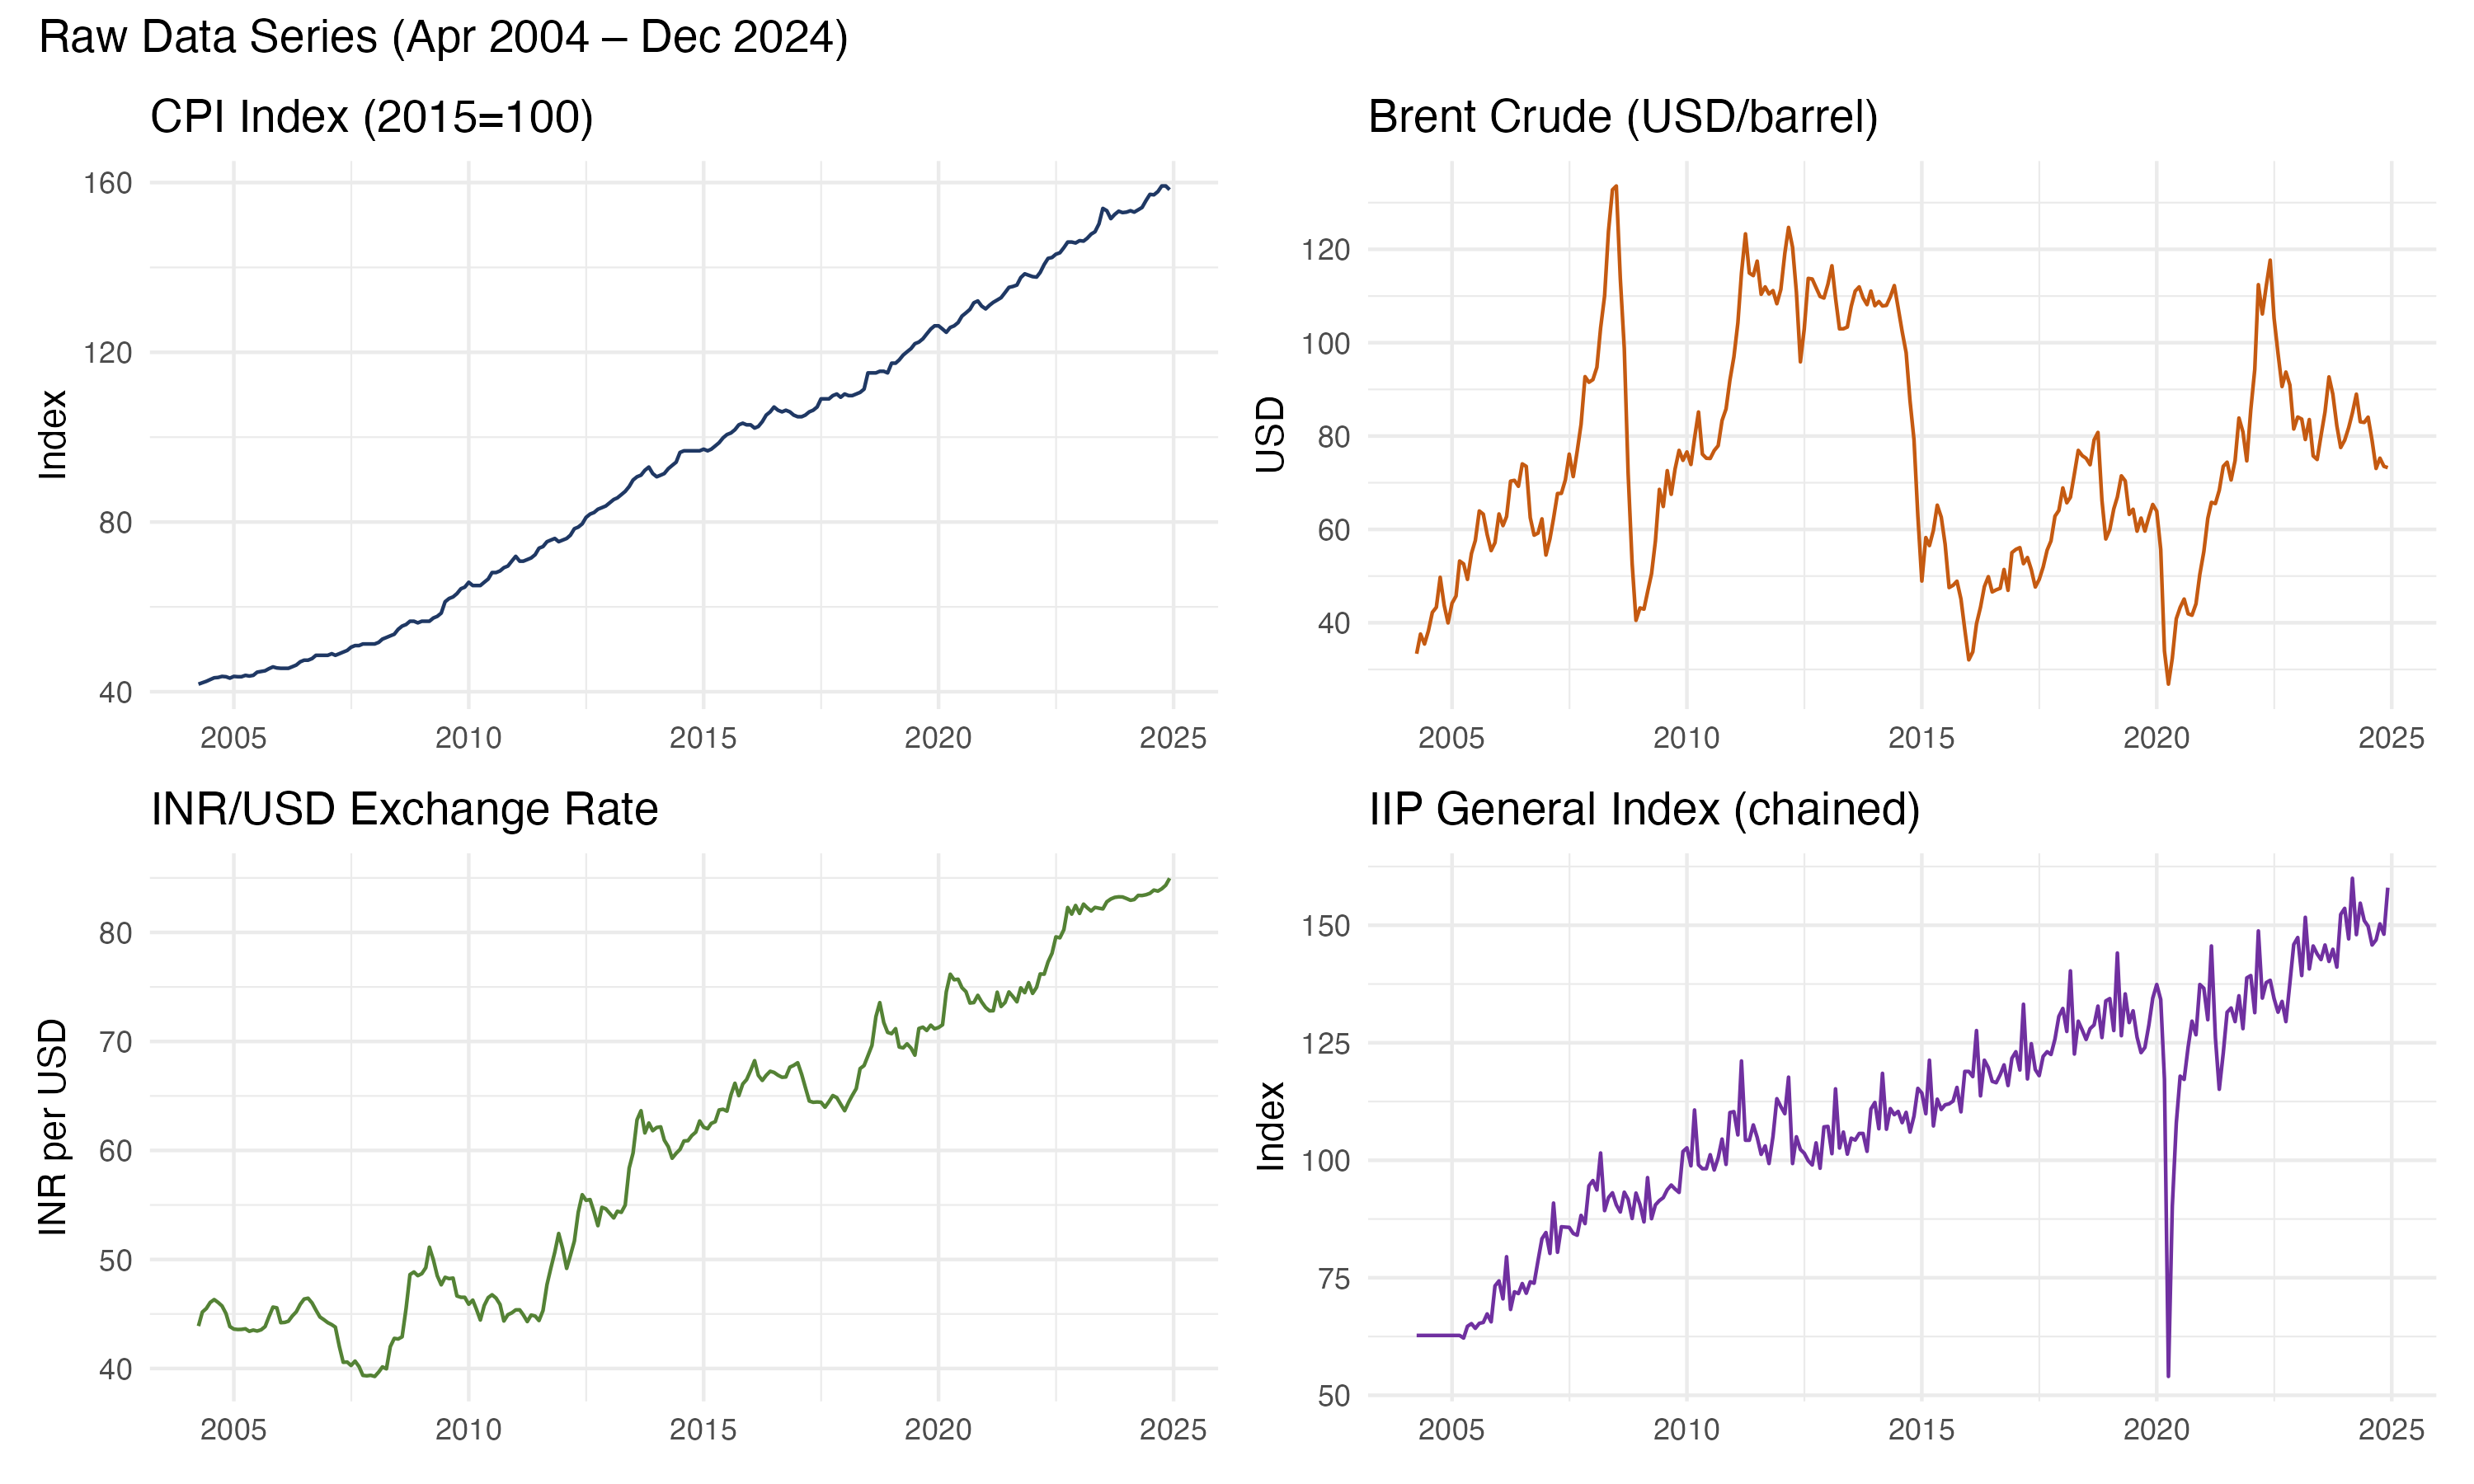
\includegraphics[width=\textwidth]{outputs/figures/fig_1_raw_series.png}
\caption{Raw data series (April 2004 to December 2024)}
\label{fig:rawseries}
\end{figure}

\begin{figure}[H]
\centering
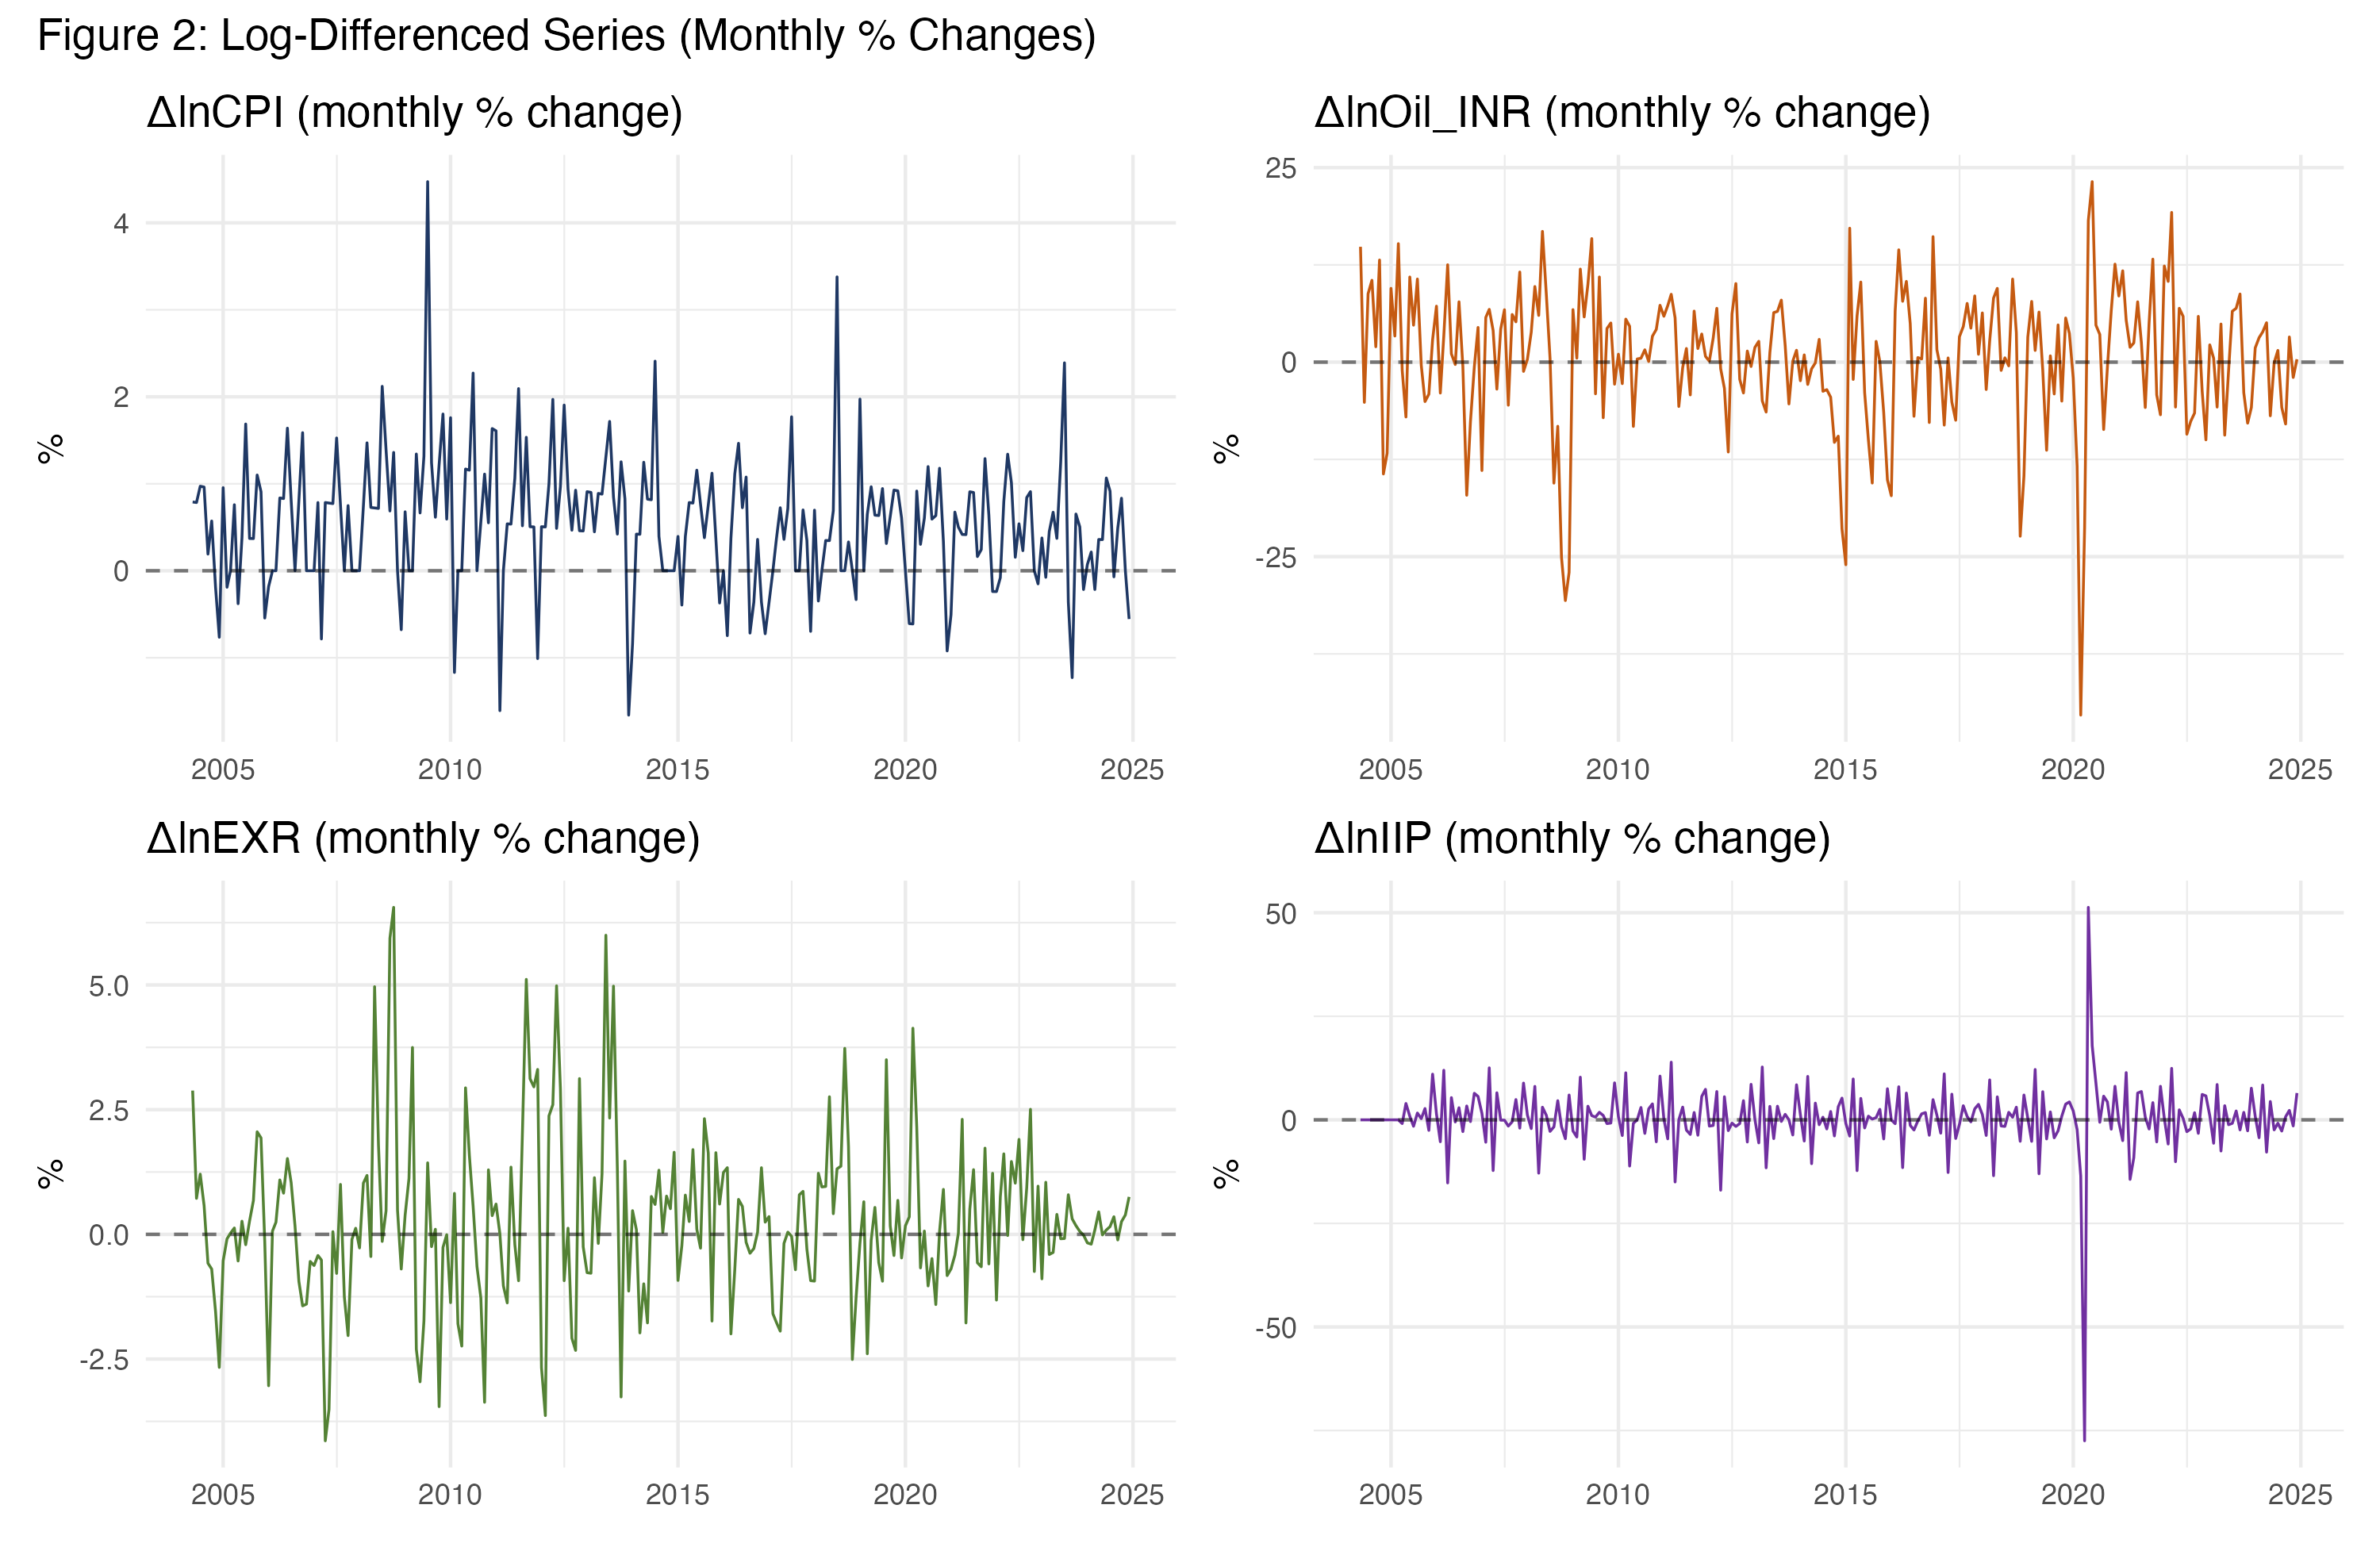
\includegraphics[width=\textwidth]{outputs/figures/fig_2_log_diff_series.png}
\caption{Log-differenced series (monthly percentage changes)}
\label{fig:logdiff}
\end{figure}


% ═══════════════════════════════════════════════════
\section{Variable construction}
% ═══════════════════════════════════════════════════

All variables are converted to monthly percentage changes using log-differences multiplied by 100:
\begin{equation}
\Delta \ln X_t = 100 \times \left[\ln(X_t) - \ln(X_{t-1})\right]
\end{equation}

Since India imports oil, the relevant price for consumers is in rupees, not dollars. So we construct:
\begin{equation}
\text{Oil\_INR}_t = \text{Brent\_USD}_t \times \text{EXR}_t
\end{equation}

This way the oil variable captures both the world oil price and the exchange rate in one series. When the rupee weakens, Oil\_INR goes up even if Brent stays flat.

The key step for testing asymmetry is splitting the oil change into positive and negative parts:
\begin{align}
\Delta \ln \text{Oil}^{+}_t &= \max\!\left(\Delta \ln \text{Oil}_t,\; 0\right) \\[4pt]
\Delta \ln \text{Oil}^{-}_t &= \min\!\left(\Delta \ln \text{Oil}_t,\; 0\right)
\end{align}

The negative component stays negative. So if oil fell by 10\%, then $\Delta\ln\text{Oil}^-_t = -10$ and $\Delta\ln\text{Oil}^+_t = 0$.

Figure~\ref{fig:oildecomp} shows the cumulative partial sums of these two components over time.

\begin{figure}[H]
\centering
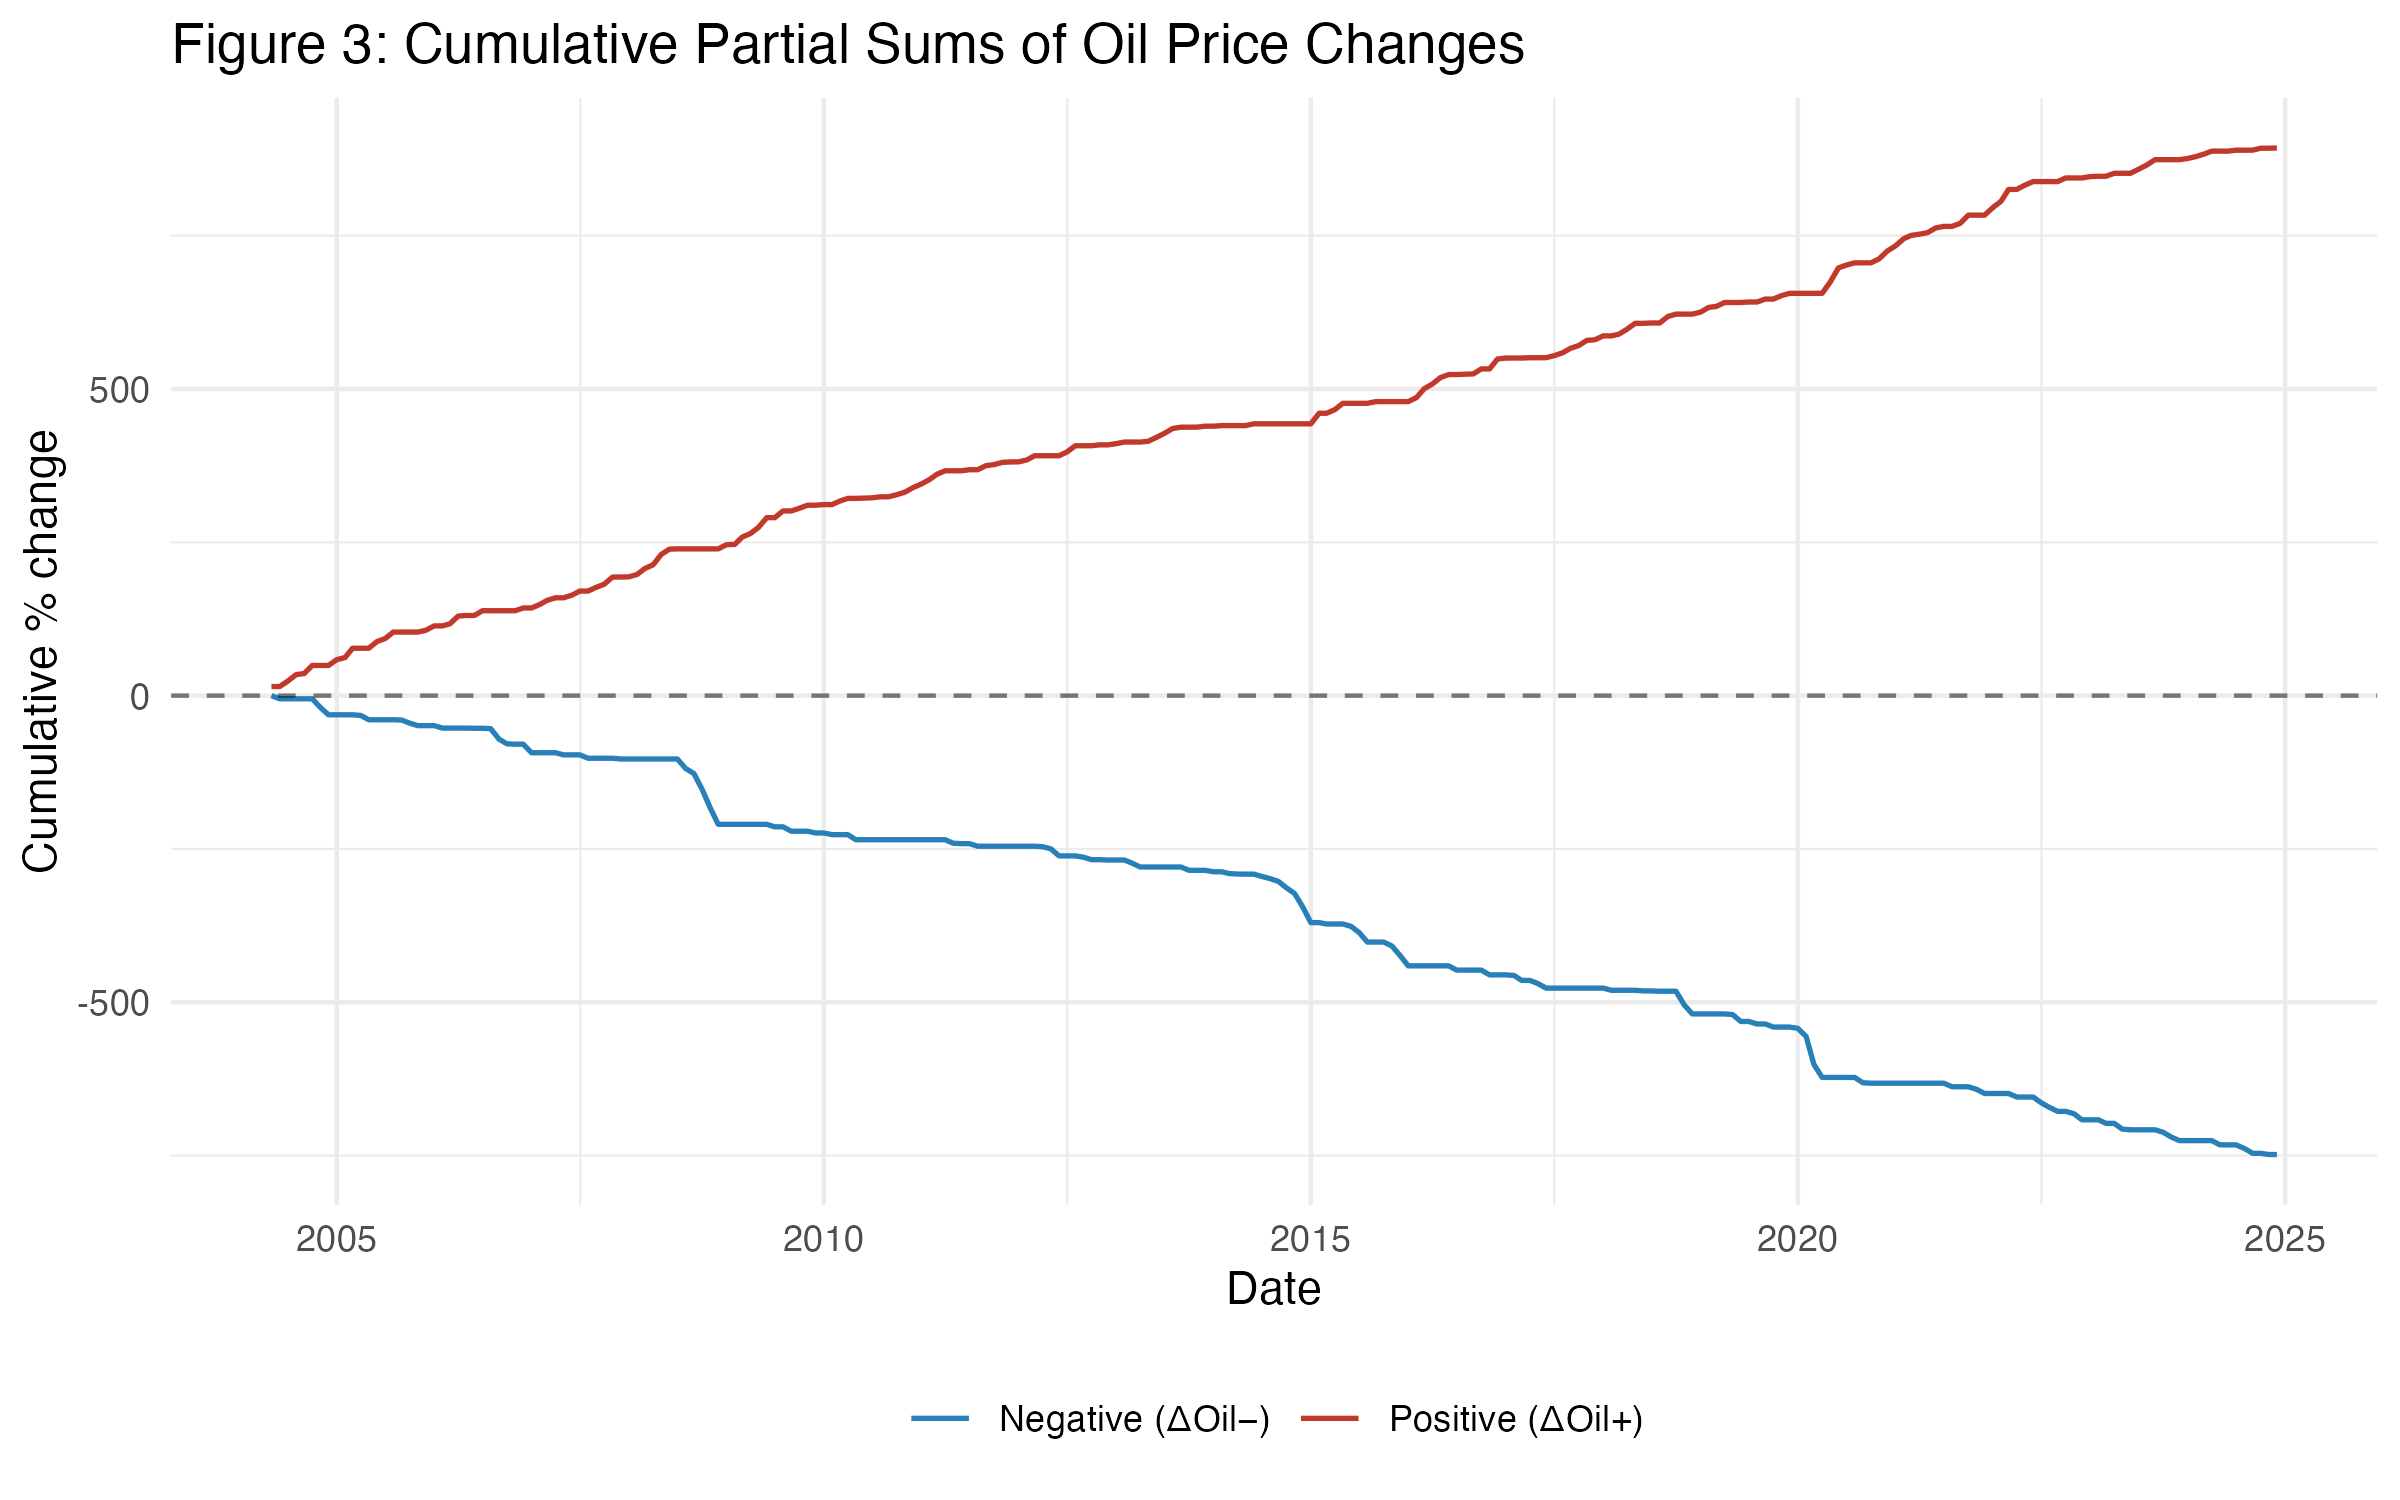
\includegraphics[width=0.85\textwidth]{outputs/figures/fig_3_oil_decomposition.png}
\caption{Cumulative partial sums of positive and negative oil price changes}
\label{fig:oildecomp}
\end{figure}

Three dummy variables control for structural breaks:
\begin{itemize}[noitemsep]
\item $D_{\text{petrol}} = 1$ from June 2010 (petrol price deregulation)
\item $D_{\text{diesel}} = 1$ from October 2014 (diesel price deregulation)
\item $D_{\text{COVID}} = 1$ for April 2020 only (lockdown outlier)
\end{itemize}

Eleven monthly dummies ($M_1$ to $M_{11}$, with December as reference) capture seasonal patterns.


% ═══════════════════════════════════════════════════
\section{Unit root tests}
% ═══════════════════════════════════════════════════

Before estimating the ADL models, the ADF test is used to check whether the variables are stationary. Table~\ref{tab:adf} shows the results.

\begin{table}[H]
\centering
\caption{ADF unit root test results}
\label{tab:adf}
\small
\begin{tabular}{lcccl}
\toprule
\textbf{Variable} & \textbf{ADF stat.} & \textbf{Lags} & \textbf{$p$-value} & \textbf{Conclusion} \\
\midrule
$\ln(\text{CPI})$      & $-$0.320 & 6 & 0.990 & Non-stationary \\
$\ln(\text{Oil\_INR})$  & $-$2.574 & 6 & 0.334 & Non-stationary \\
$\ln(\text{EXR})$       & $-$3.686 & 6 & 0.025 & Stationary \\
$\ln(\text{IIP})$       & $-$3.200 & 6 & 0.088 & Borderline \\
\midrule
$\Delta\ln\text{CPI}$  & $-$9.042 & 6 & $<$0.01 & Stationary \\
$\Delta\ln\text{Oil}$  & $-$6.128 & 6 & $<$0.01 & Stationary \\
$\Delta\ln\text{EXR}$  & $-$5.210 & 6 & $<$0.01 & Stationary \\
$\Delta\ln\text{IIP}$  & $-$8.221 & 6 & $<$0.01 & Stationary \\
\bottomrule
\end{tabular}
\end{table}

Log-CPI and log-Oil\_INR are clearly non-stationary in levels. All first-differenced series are stationary ($p < 0.01$). This confirms that working with log-differences is appropriate.


% ═══════════════════════════════════════════════════
\section{Model specification and estimation}
% ═══════════════════════════════════════════════════

\subsection{Symmetric ADL benchmark}

A simple symmetric ADL(1,1) is estimated first as a benchmark:
\begin{equation}
\Delta\ln\text{CPI}_t = \alpha + \gamma_1 \Delta\ln\text{CPI}_{t-1} + \beta_0 \Delta\ln\text{Oil}_t + \beta_1 \Delta\ln\text{Oil}_{t-1} + \delta\,\Delta\ln\text{IIP}_t + \mathbf{D}'\boldsymbol{\phi} + \varepsilon_t
\end{equation}

The cumulative pass-through is $\text{CPT} = \beta_0 + \beta_1 = 0.0028$, which is basically zero ($F = 0.31$, $p = 0.578$). The symmetric model suggests oil does not matter for CPI at all. But this could be because positive and negative effects cancel each other out in the aggregate.

\subsection{Main asymmetric ADL model}

The main model allows positive and negative oil shocks to have different effects:
\begin{equation}
\begin{aligned}
\Delta\ln\text{CPI}_t = \alpha &+ \sum_{i=1}^{p}\gamma_i\,\Delta\ln\text{CPI}_{t-i} + \sum_{j=0}^{3}\pi^+_j\,\Delta\ln\text{Oil}^+_{t-j} \\
&+ \sum_{j=0}^{3}\pi^-_j\,\Delta\ln\text{Oil}^-_{t-j} + \delta\,\Delta\ln\text{IIP}_t + \mathbf{D}'\boldsymbol{\phi} + \varepsilon_t
\end{aligned}
\end{equation}

The oil lag length is fixed at $q = 3$ months, which is standard for monthly pass-through studies. The AR lag order $p$ is selected by AIC from $\{1, 2, 3, 4\}$.

To make the AIC comparison fair, all four candidate models are estimated on the same common sample (determined by the most demanding model, $p = 4$). After selecting $p$, the final model is re-estimated on the maximal sample implied by that $p$.

\begin{table}[H]
\centering
\caption{AIC-based AR lag selection}
\label{tab:aicselection}
\small
\begin{tabular}{ccc}
\toprule
\textbf{AR lags ($p$)} & \textbf{AIC} & \textbf{Selected?} \\
\midrule
1 & 440.88 & \\
2 & 441.62 & \\
3 & \textbf{437.80} & $\leftarrow$ Yes \\
4 & 439.77 & \\
\bottomrule
\end{tabular}
\end{table}

$p = 3$ gives the lowest AIC, so the main model is an \textbf{ADL(3,3)}.

\subsection{Inference}

All $t$-tests and $F$-tests use the Newey-West HAC covariance estimator with bandwidth $L = \lfloor 0.75 \times n^{1/3} \rfloor = 4$. This corrects for heteroskedasticity and possible serial correlation in the residuals.


% ═══════════════════════════════════════════════════
\section{Results}
% ═══════════════════════════════════════════════════

\subsection{Coefficient estimates}

Table~\ref{tab:asymresults} reports the main ADL(3,3) results.

\begin{table}[H]
\centering
\caption{Asymmetric ADL(3,3) results, headline CPI}
\label{tab:asymresults}
\small
\begin{tabular}{L{3.8cm}R{1.5cm}R{1.3cm}R{1.2cm}R{1.2cm}c}
\toprule
\textbf{Variable} & \textbf{Coeff.} & \textbf{NW SE} & \textbf{$t$} & \textbf{$p$} & \\
\midrule
\multicolumn{6}{l}{\textit{CPI lags}} \\
$\Delta\ln\text{CPI}_{t-1}$      & 0.1652 & 0.0575 & 2.88 & 0.004 & *** \\
$\Delta\ln\text{CPI}_{t-2}$      & $-$0.0785 & 0.0688 & $-$1.14 & 0.255 & \\
$\Delta\ln\text{CPI}_{t-3}$      & $-$0.1159 & 0.0677 & $-$1.71 & 0.088 & * \\
\midrule
\multicolumn{6}{l}{\textit{Positive oil shocks ($\pi^+$)}} \\
$\Delta\ln\text{Oil}^{+}_{t}$    & $-$0.0040 & 0.0073 & $-$0.55 & 0.580 & \\
$\Delta\ln\text{Oil}^{+}_{t-1}$  & 0.0054 & 0.0114 & 0.48 & 0.635 & \\
$\Delta\ln\text{Oil}^{+}_{t-2}$  & 0.0143 & 0.0086 & 1.66 & 0.099 & * \\
$\Delta\ln\text{Oil}^{+}_{t-3}$  & 0.0056 & 0.0073 & 0.77 & 0.441 & \\
\midrule
\multicolumn{6}{l}{\textit{Negative oil shocks ($\pi^-$)}} \\
$\Delta\ln\text{Oil}^{-}_{t}$    & 0.0099 & 0.0068 & 1.44 & 0.151 & \\
$\Delta\ln\text{Oil}^{-}_{t-1}$  & $-$0.0077 & 0.0084 & $-$0.91 & 0.362 & \\
$\Delta\ln\text{Oil}^{-}_{t-2}$  & $-$0.0066 & 0.0083 & $-$0.78 & 0.433 & \\
$\Delta\ln\text{Oil}^{-}_{t-3}$  & 0.0050 & 0.0061 & 0.82 & 0.414 & \\
\midrule
\multicolumn{6}{l}{\textit{Controls}} \\
$\Delta\ln\text{IIP}_{t}$        & $-$0.0076 & 0.0052 & $-$1.45 & 0.148 & \\
$D_{\text{petrol}}$              & 0.1163 & 0.1135 & 1.02 & 0.307 & \\
$D_{\text{diesel}}$              & $-$0.3385 & 0.0915 & $-$3.70 & 0.000 & *** \\
$D_{\text{COVID}}$               & $-$0.3446 & 0.5182 & $-$0.66 & 0.507 & \\
\midrule
Adj.\ $R^2$ & 0.4492 &&&& \\
$N$          & 245    &&&& \\
\bottomrule
\multicolumn{6}{l}{\footnotesize *** $p<0.01$, ** $p<0.05$, * $p<0.10$. Newey-West HAC SEs.} \\
\multicolumn{6}{l}{\footnotesize Monthly dummies $M_1$ to $M_{11}$ included but not shown.} \\
\end{tabular}
\end{table}

The first CPI lag is significant, meaning past inflation predicts current inflation. Among the positive oil coefficients, the two-month lag ($\pi^+_2 = 0.0143$) is the largest and marginally significant. The contemporaneous coefficient is slightly negative, which suggests it takes a month or two for oil price increases to show up in CPI. None of the negative oil coefficients are individually significant.

The diesel deregulation dummy is significant with a negative coefficient ($-$0.3385), meaning monthly inflation was about 0.34 percentage points lower on average after diesel was deregulated in October 2014.

\subsection{Cumulative pass-through}

The individual lag coefficients are noisy. What matters more is the cumulative pass-through, which sums the coefficients across all lags:
\begin{align}
\text{CPT}^+ &= \pi^+_0 + \pi^+_1 + \pi^+_2 + \pi^+_3 = \mathbf{0.0213} \\[4pt]
\text{CPT}^- &= \pi^-_0 + \pi^-_1 + \pi^-_2 + \pi^-_3 = \mathbf{0.0006}
\end{align}

A \textbf{+10\% oil shock} raises monthly CPI inflation by $0.0213 \times 10 = +0.213$ percentage points.\\
A \textbf{$-$10\% oil shock} changes CPI by $0.0006 \times (-10) = -0.006$ percentage points (basically nothing).

Table~\ref{tab:waldtests} shows the Wald test results for the cumulative restrictions.

\begin{table}[H]
\centering
\caption{Cumulative pass-through and Wald tests (HAC)}
\label{tab:waldtests}
\small
\begin{tabular}{L{4cm}R{1.5cm}R{1.3cm}R{1.3cm}l}
\toprule
\textbf{Hypothesis} & \textbf{Value} & \textbf{$F$} & \textbf{$p$} & \textbf{5\% decision} \\
\midrule
$H_0$: CPT$^+ = 0$        & 0.0213 & 2.410 & 0.122 & Fail to reject \\
$H_0$: CPT$^- = 0$        & 0.0006 & 0.006 & 0.938 & Fail to reject \\
$H_0$: CPT$^+ =$ CPT$^-$  &        & 1.384 & 0.241 & Fail to reject \\
\midrule
$+10\%$ oil shock effect   & \multicolumn{4}{l}{$+$0.213 pp on monthly CPI} \\
$-10\%$ oil shock effect   & \multicolumn{4}{l}{$-$0.006 pp on monthly CPI} \\
\bottomrule
\end{tabular}
\end{table}

The point estimates look asymmetric. CPT$^+$ is about 35 times larger than $|$CPT$^-|$. But the Wald test for asymmetry does not reject at 5\% ($p = 0.241$). So the direction of asymmetry is present in the data, but the statistical evidence is not strong enough. This is actually quite common with headline CPI, because the CPI basket in India has about 46\% weight on food, and food prices are driven by monsoons and supply issues rather than oil.

Figure~\ref{fig:cpt} shows how the cumulative pass-through builds up over the lag horizons.

\begin{figure}[H]
\centering
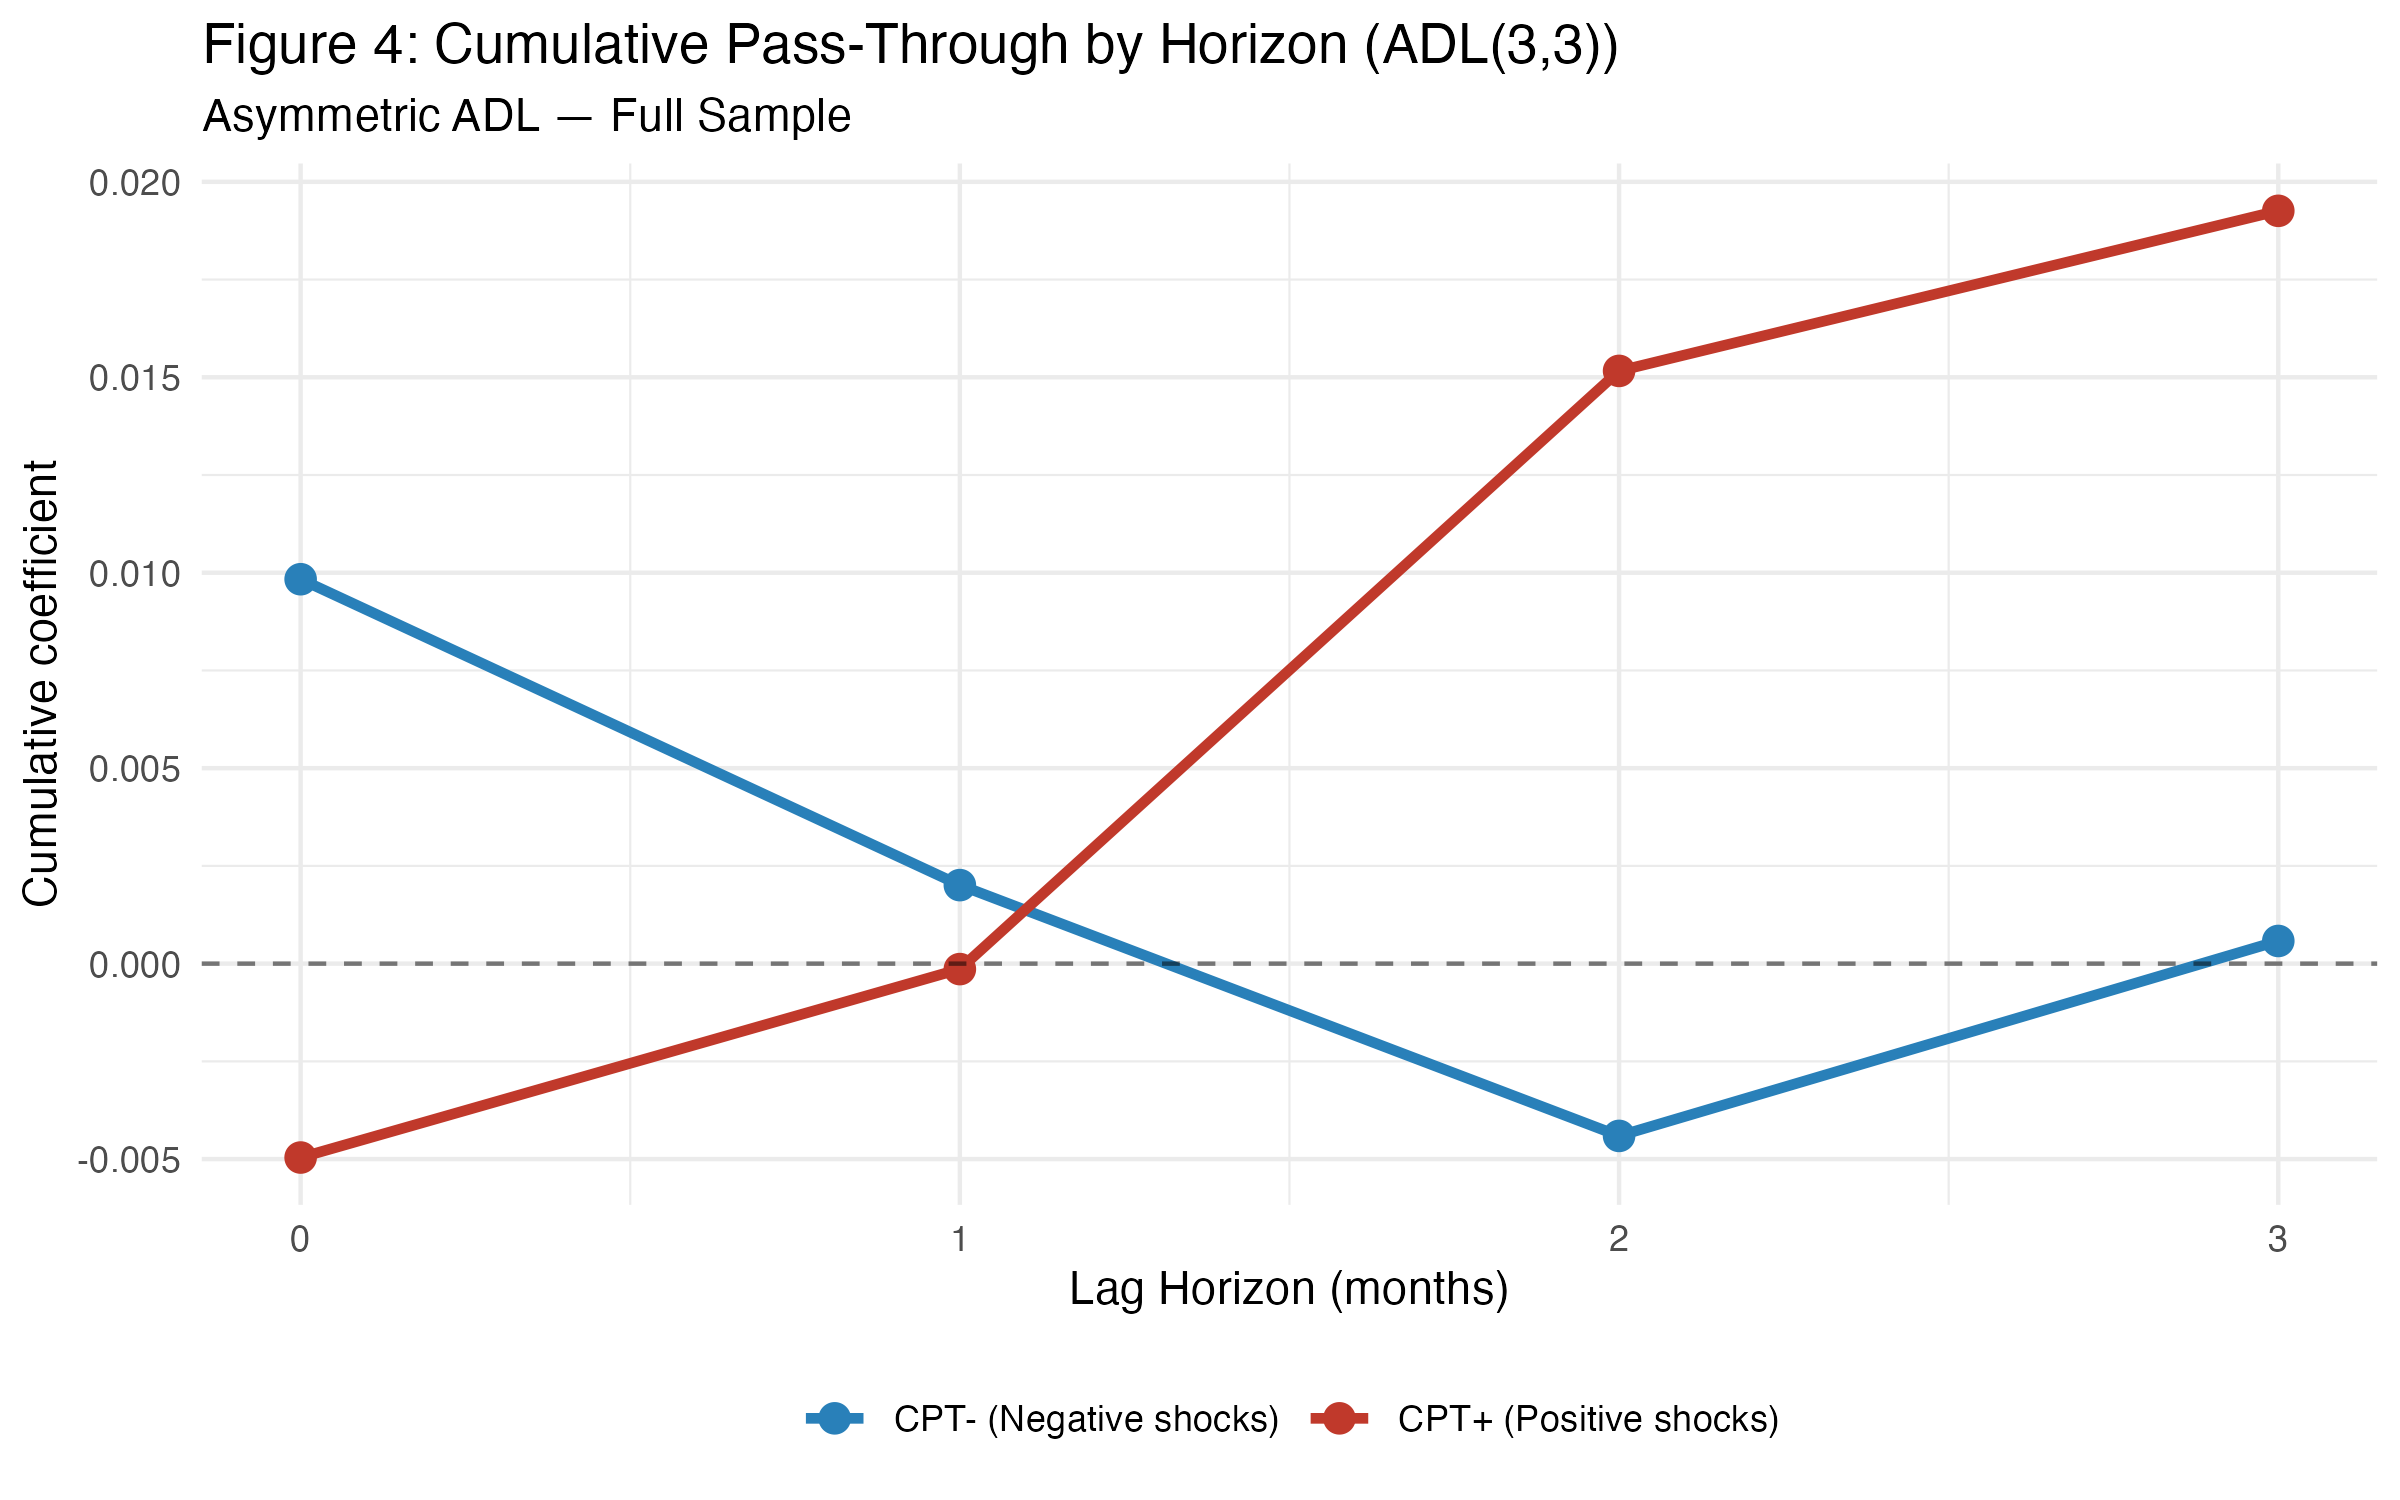
\includegraphics[width=0.85\textwidth]{outputs/figures/fig_4_cumulative_passthrough.png}
\caption{Cumulative pass-through by lag horizon, ADL(3,3)}
\label{fig:cpt}
\end{figure}


% ═══════════════════════════════════════════════════
\section{Diagnostic tests}
\label{sec:diagnostics}
% ═══════════════════════════════════════════════════

Table~\ref{tab:diagnostics} reports the diagnostic tests for the main model.

\begin{table}[H]
\centering
\caption{Diagnostic tests for the ADL(3,3) model}
\label{tab:diagnostics}
\small
\begin{tabular}{L{4.5cm}R{1.5cm}R{1.3cm}L{4.5cm}}
\toprule
\textbf{Test} & \textbf{Stat.} & \textbf{$p$} & \textbf{Result} \\
\midrule
Breusch-Godfrey (12 lags) & 19.71 & 0.073 & Pass, no serial correlation \\

Ramsey RESET               & 2.80  & 0.063 & Pass, no misspecification \\
CUSUM stability            & 0.86  & 0.091 & Pass, parameters stable \\
\bottomrule
\end{tabular}
\end{table}

The Breusch-Godfrey test passes, meaning the AR lags are doing a good job of absorbing serial correlation. The RESET test passes, confirming the linear specification is adequate. The CUSUM test passes, indicating stable parameters.

\begin{figure}[H]
\centering
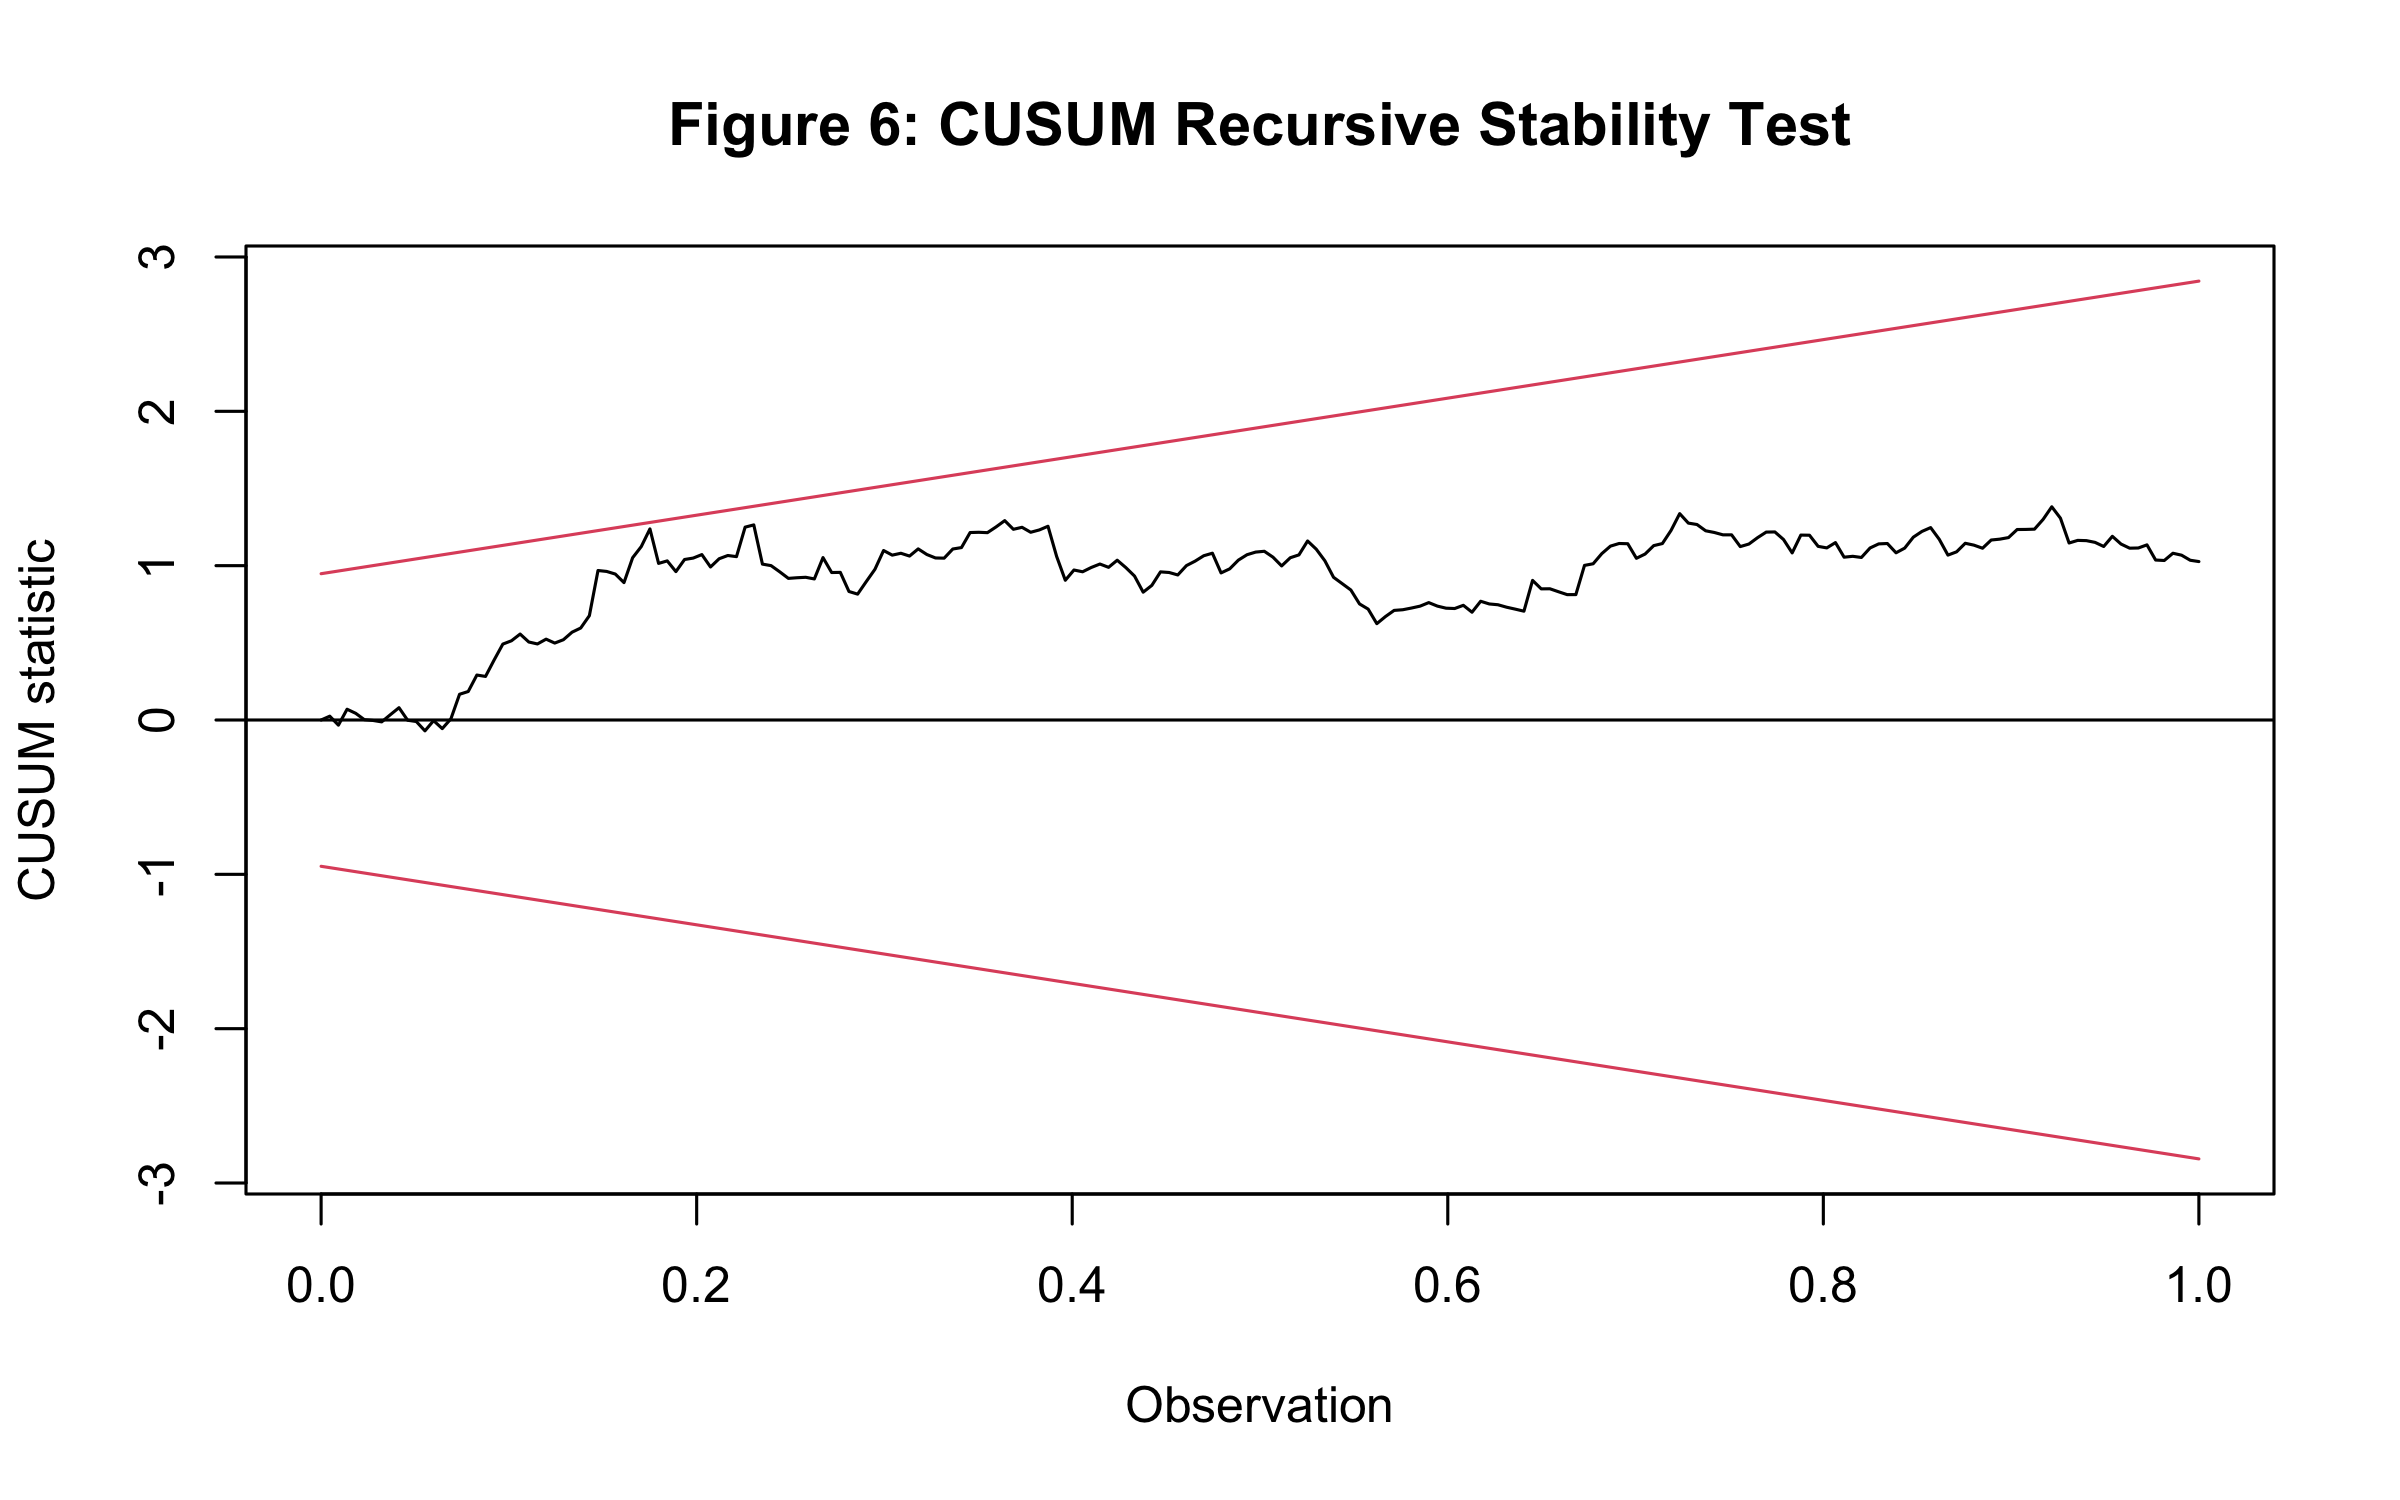
\includegraphics[width=0.85\textwidth]{outputs/figures/fig_6_cusum_stability.png}
\caption{CUSUM recursive stability test}
\label{fig:cusum}
\end{figure}

\begin{figure}[H]
\centering
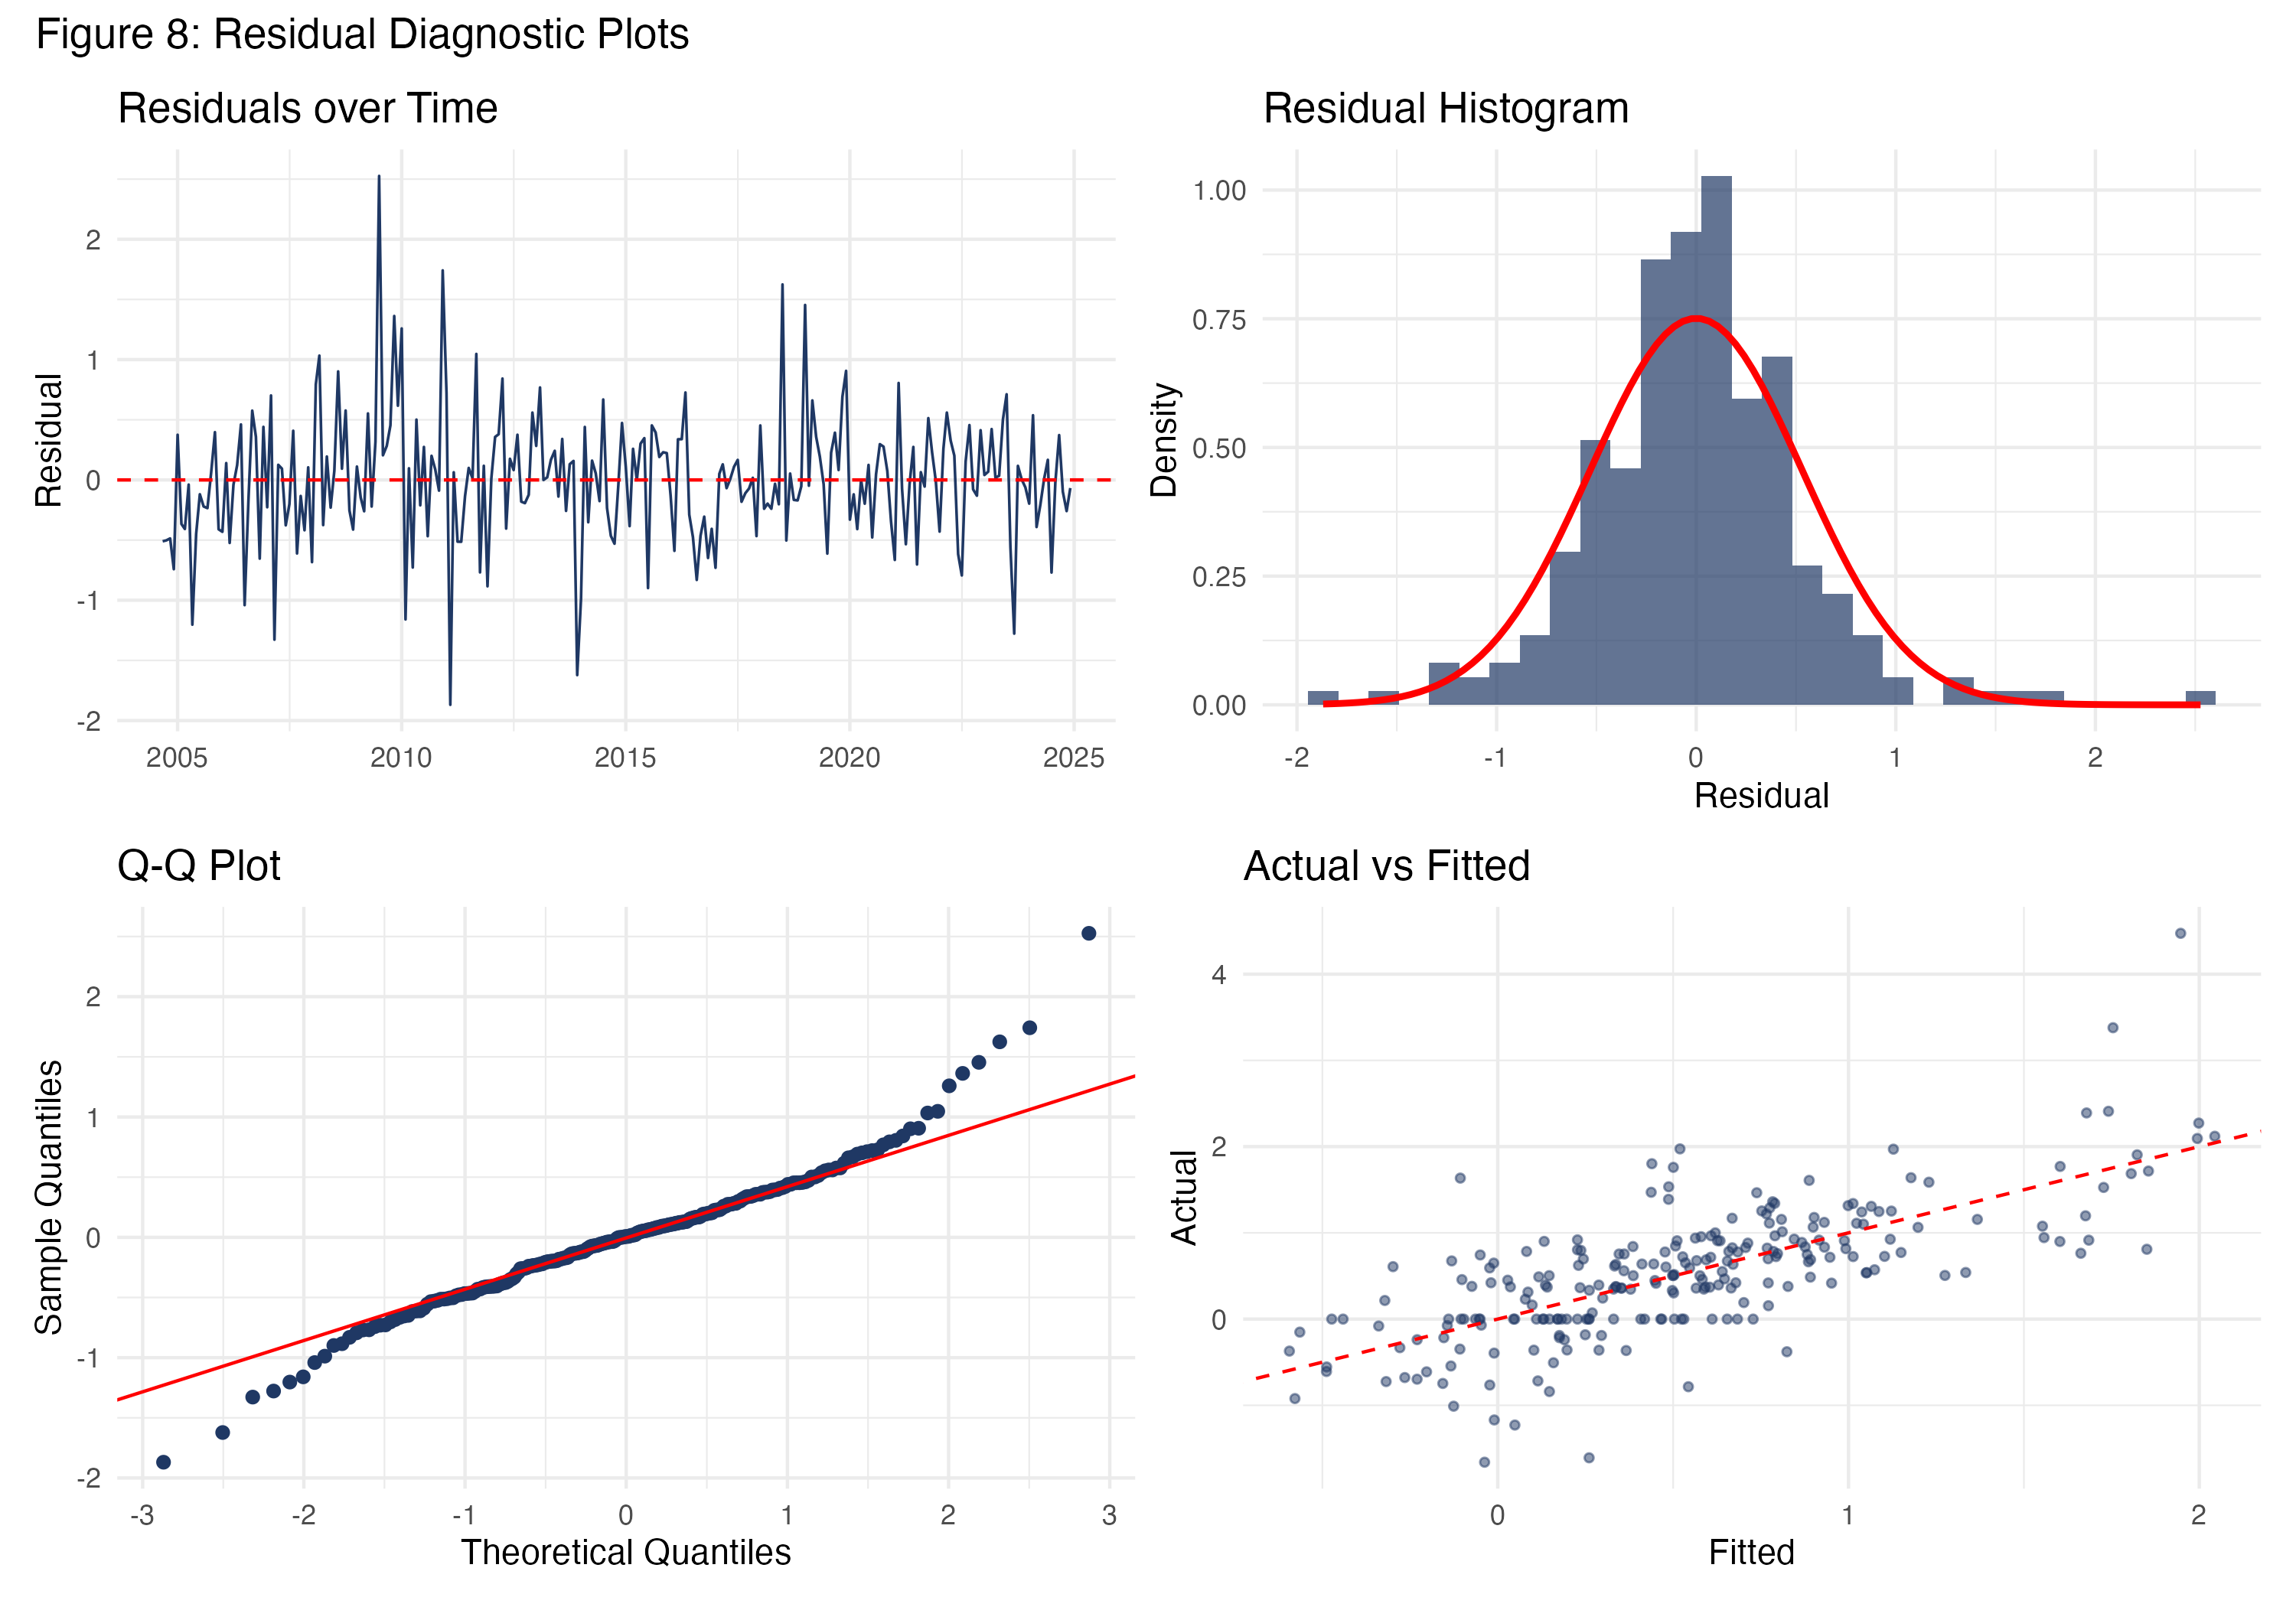
\includegraphics[width=\textwidth]{outputs/figures/fig_8_residual_diagnostics.png}
\caption{Residual diagnostic plots}
\label{fig:residuals}
\end{figure}


% ═══════════════════════════════════════════════════
\section{Sub-sample analysis}
% ═══════════════════════════════════════════════════

The sample is split at October 2014 (diesel deregulation) to check whether the pass-through changed after fuel pricing was freed.

\begin{table}[H]
\centering
\caption{Sub-sample comparison}
\label{tab:subsample}
\small
\begin{tabular}{L{5cm}R{1cm}R{1.5cm}R{1.5cm}R{1.4cm}R{1.3cm}}
\toprule
\textbf{Period} & \textbf{$N$} & \textbf{CPT$^{+}$} & \textbf{CPT$^{-}$} & \textbf{$p$(asym)} & \textbf{Adj.~$R^2$} \\
\midrule
Pre-2014  & 122 & 0.0173 & 0.0099  & 0.846 & 0.357 \\
Post-2014 & 123 & 0.0102 & $-$0.0020 & 0.443 & 0.500 \\
\bottomrule
\end{tabular}
\end{table}

In both sub-samples, CPT$^+$ is larger than CPT$^-$. The post-2014 period has a slightly negative CPT$^-$, meaning oil price falls now have a small correct-direction effect on CPI. Neither sub-sample gives a significant asymmetry test, which is expected given the smaller sample sizes.

\begin{figure}[H]
\centering
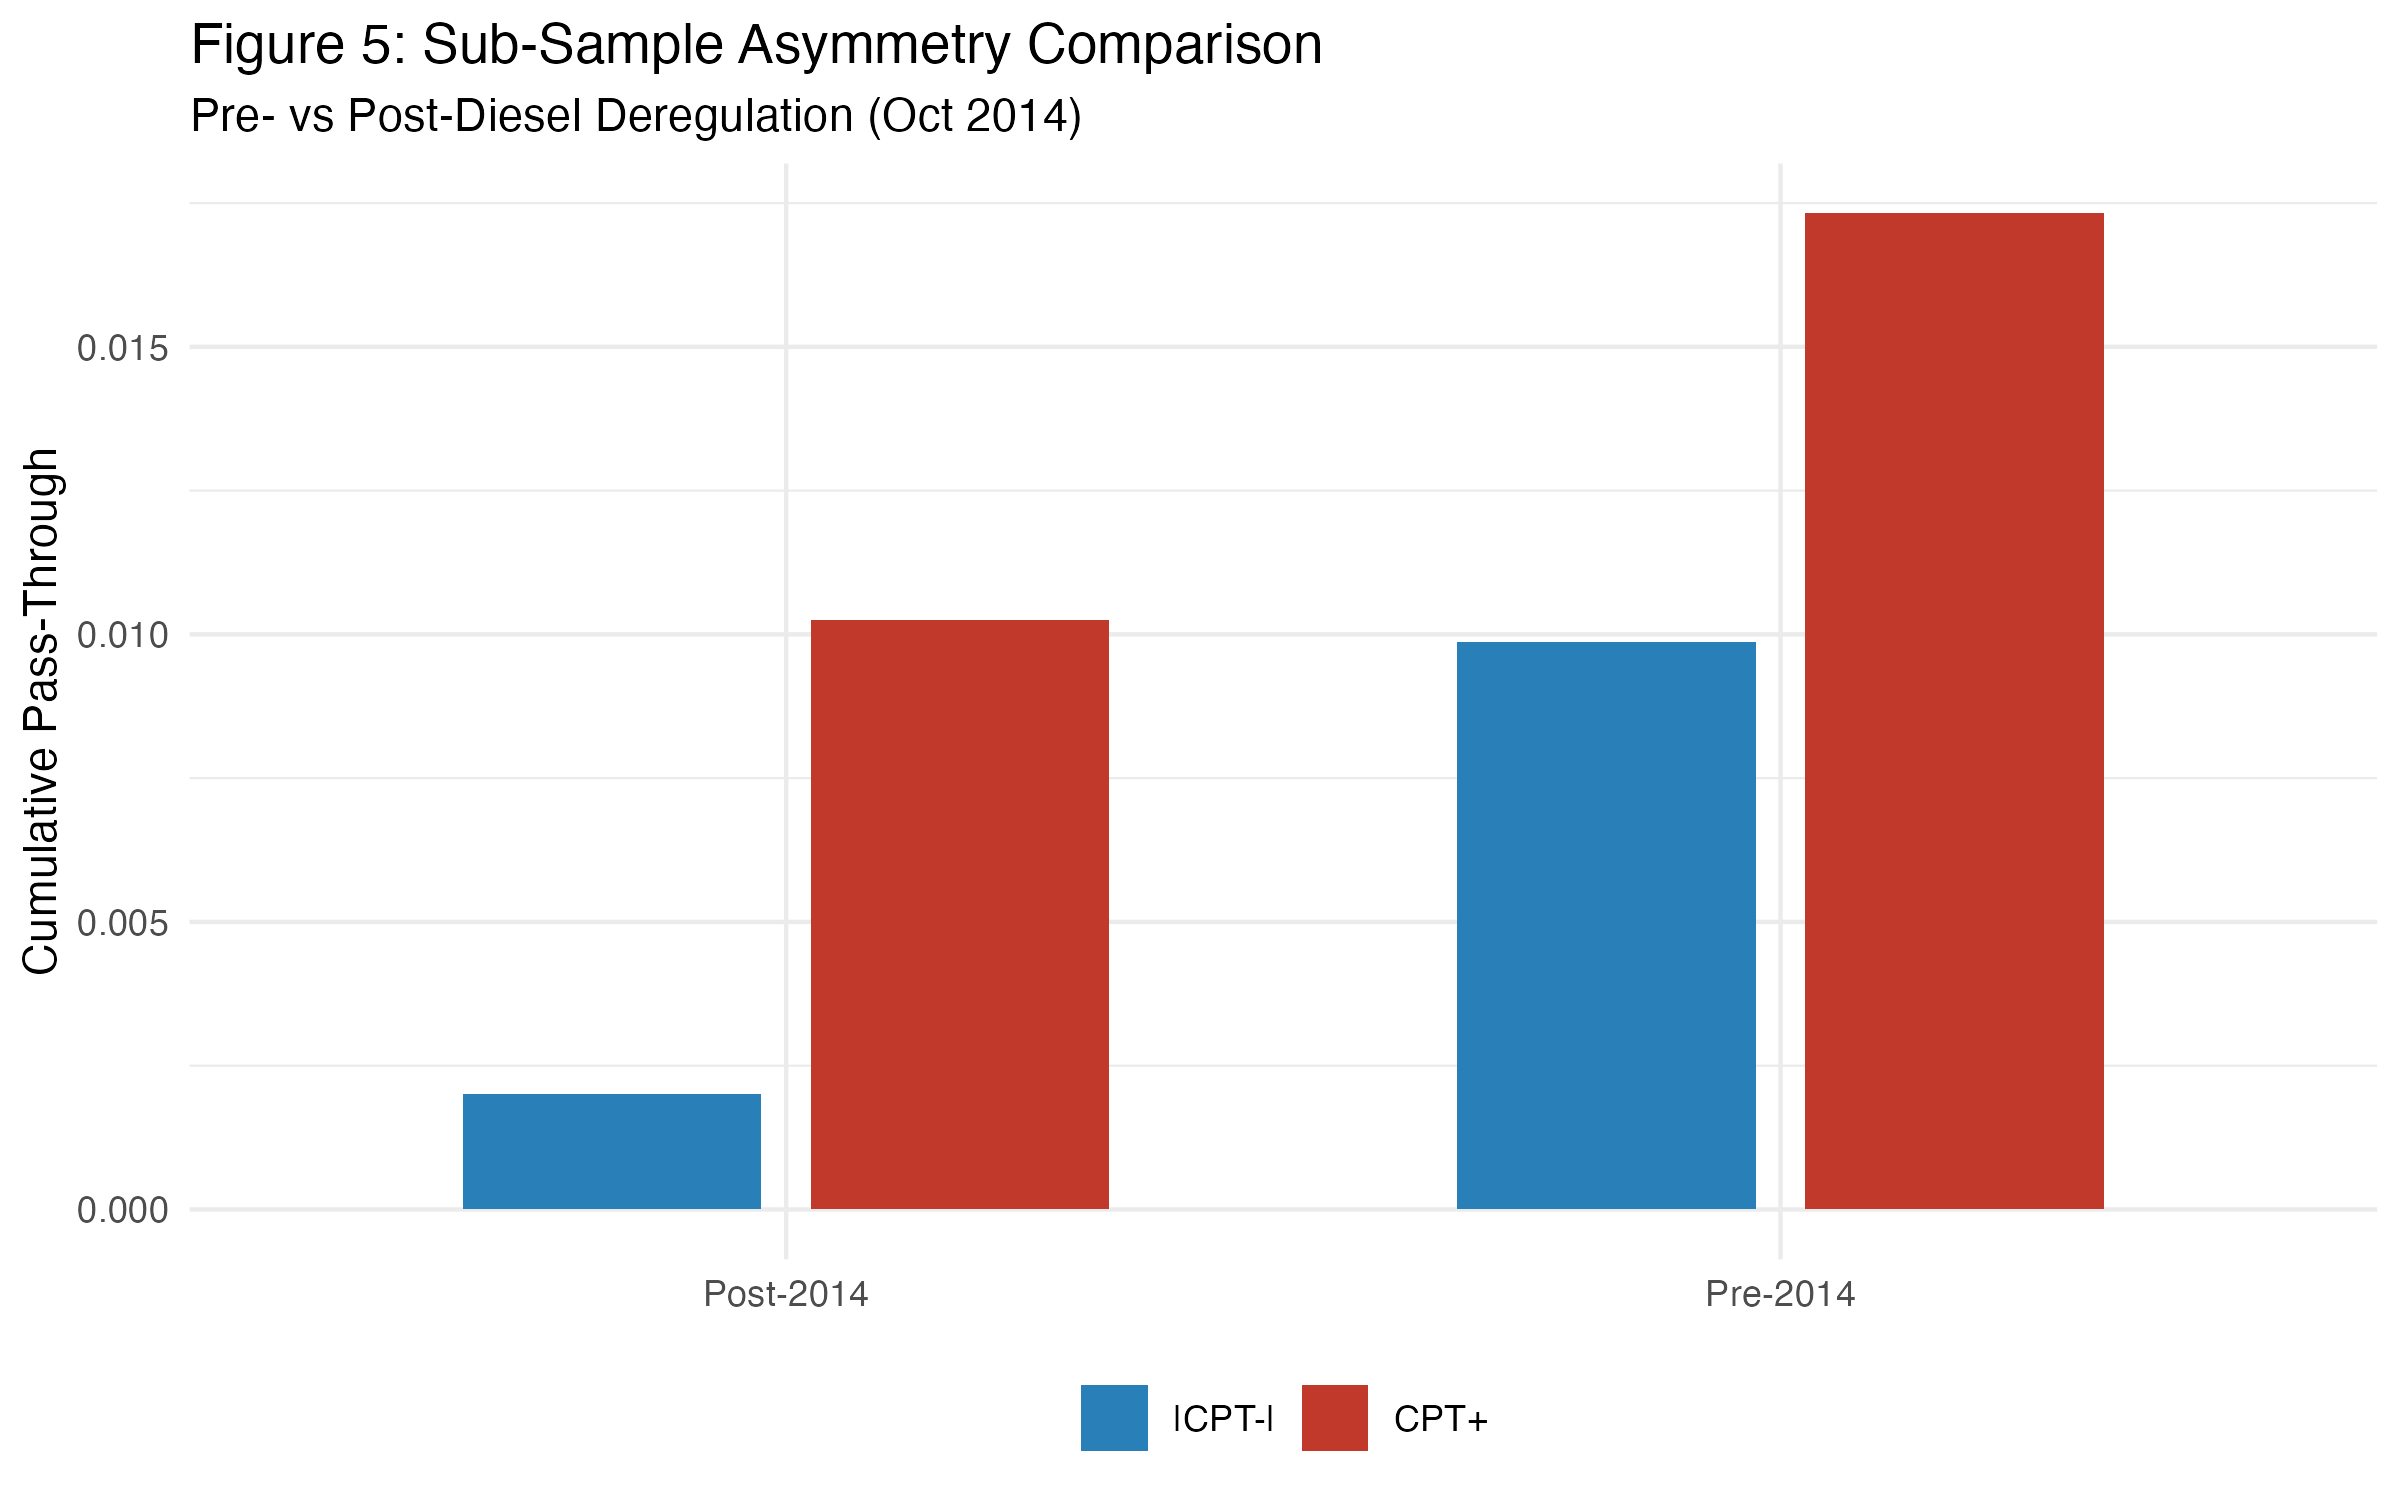
\includegraphics[width=0.78\textwidth]{outputs/figures/fig_5_subsample_comparison.png}
\caption{Sub-sample comparison of CPT$^+$ and $|$CPT$^-|$}
\label{fig:subsample}
\end{figure}


% ═══════════════════════════════════════════════════
\section{Robustness checks}
% ═══════════════════════════════════════════════════

\subsection{Brent + exchange rate specification}

Instead of using Oil\_INR, this robustness model enters Brent in USD and the exchange rate as separate variables. This lets us see how much pass-through comes from the oil price itself versus the exchange rate.

\begin{table}[H]
\centering
\caption{Brent + exchange rate robustness}
\label{tab:brentexr}
\small
\begin{tabular}{L{3.3cm}R{1.4cm}R{1.8cm}R{1.6cm}R{1.3cm}}
\toprule
\textbf{Spec.} & \textbf{CPT$^{+}$} & \textbf{$p$(CPT$^{+}$=0)} & \textbf{EXR coeff.} & \textbf{$p$(EXR)} \\
\midrule
Oil INR     & 0.0213 & 0.122 &        &       \\
Brent + EXR & 0.0275 & 0.093 & 0.0396 & 0.029 \\
\bottomrule
\end{tabular}
\end{table}

The CPT$^+$ is slightly higher in this specification (0.0275) and approaches significance at 10\%. The exchange rate coefficient is positive and significant ($p = 0.029$), confirming that rupee depreciation is an important channel for oil pass-through in India.

\subsection{Fuel and Light CPI appendix}

The same asymmetric ADL is estimated using the ``Fuel and Light'' CPI sub-group from MoSPI instead of headline CPI. This sub-group covers kerosene, LPG, and electricity, so it is more directly exposed to oil prices. The sample starts from May 2011 (164 observations).

\begin{table}[H]
\centering
\caption{Fuel and Light CPI pass-through}
\label{tab:fuellight}
\small
\begin{tabular}{L{4.5cm}R{1.5cm}R{1.5cm}l}
\toprule
\textbf{Measure} & \textbf{Value} & \textbf{$p$} & \textbf{Decision} \\
\midrule
CPT$^{+}$                     & 0.0608 & 0.034 & Significant at 5\% \\
CPT$^{-}$                     & 0.0108 & 0.665 & Not significant \\
$H_0$: CPT$^{+} =$ CPT$^{-}$ &        & 0.265 & Not significant \\
\midrule
$+10\%$ shock effect           & \multicolumn{3}{l}{$+$0.609 pp on monthly Fuel CPI} \\
\bottomrule
\end{tabular}
\end{table}

This is the strongest result in the project. CPT$^+$ is 0.061 and statistically significant at 5\% ($p = 0.034$). A 10\% oil increase raises Fuel and Light CPI by about 0.61 percentage points per month, roughly three times the headline CPI effect. This makes sense because the Fuel and Light sub-group does not include food or services, which dilute the oil signal in headline CPI.

\subsection{Rolling window}

A 60-month rolling window tracks how the pass-through changes over time.

\begin{figure}[H]
\centering
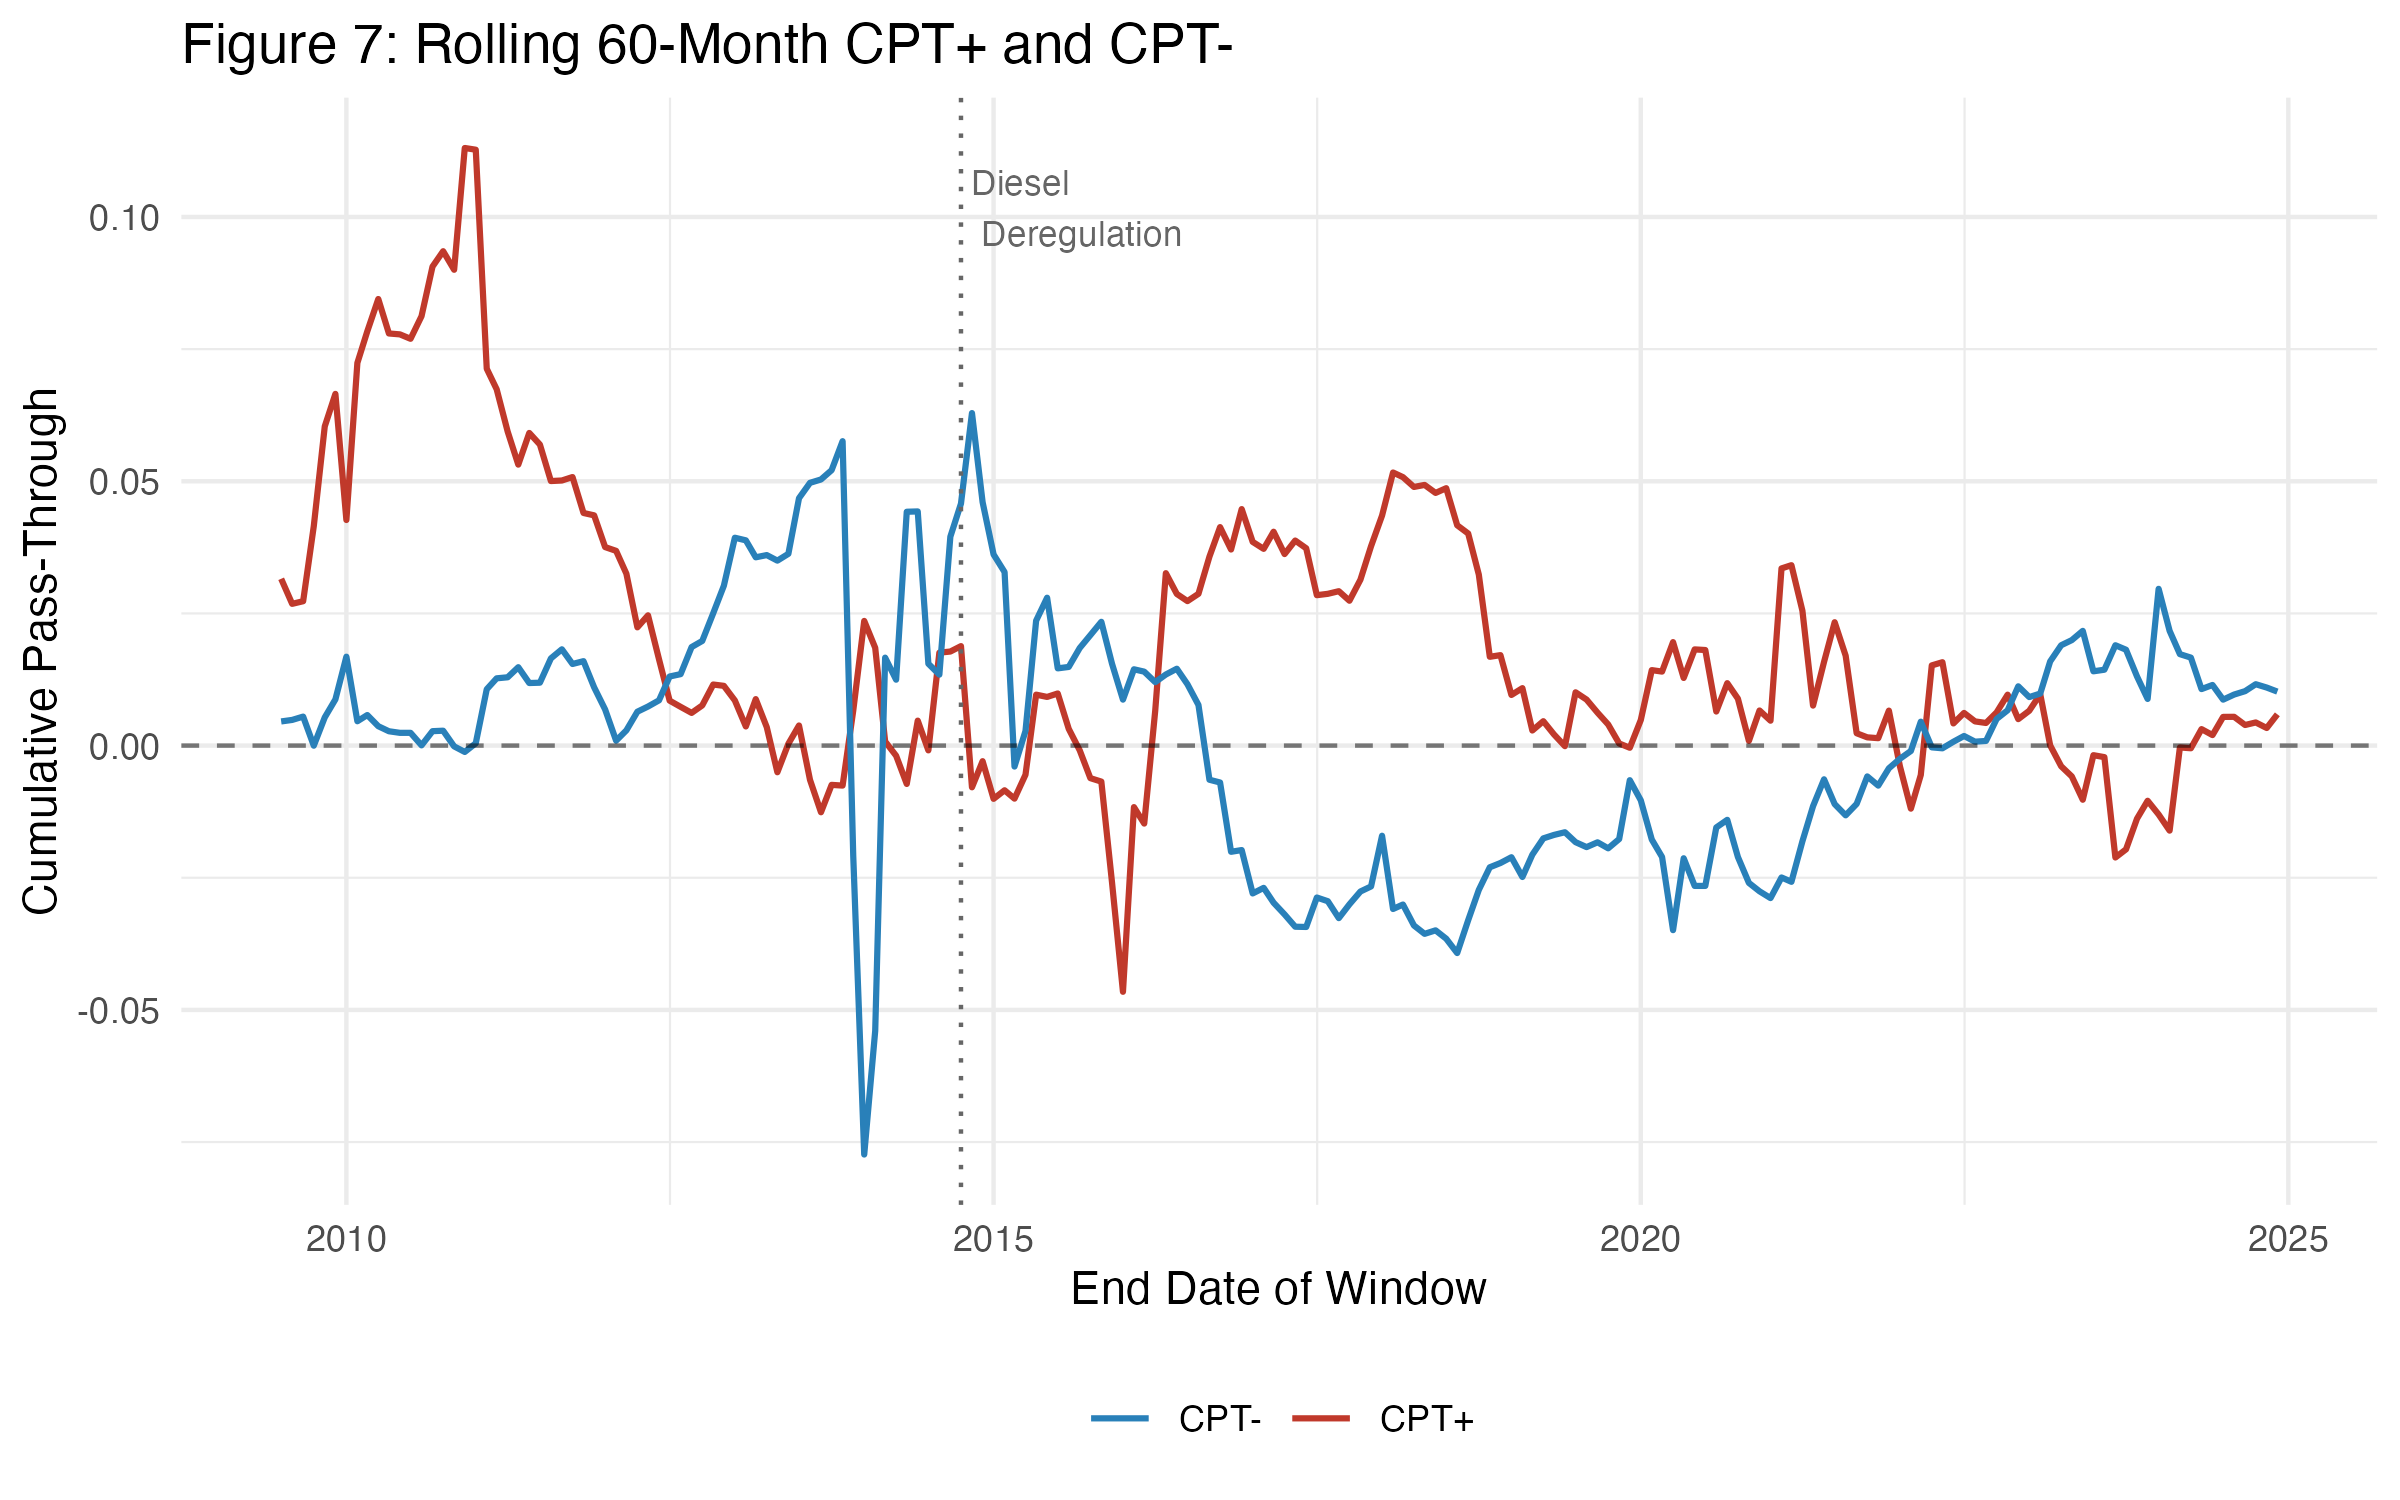
\includegraphics[width=0.85\textwidth]{outputs/figures/fig_7_rolling_window.png}
\caption{Rolling 60-month CPT$^+$ and CPT$^-$}
\label{fig:rolling}
\end{figure}

CPT$^+$ is generally above CPT$^-$ throughout the sample, though both fluctuate. The positive pass-through was higher in windows ending around 2014 to 2016 and lower after 2020.

\subsection{Other checks}

Removing the COVID dummy and winsorising the oil shock variables at the 1st and 99th percentiles both produce CPT$^+$ values close to the main estimate (around 0.02). Neither check changes the general conclusion.

\begin{figure}[H]
\centering
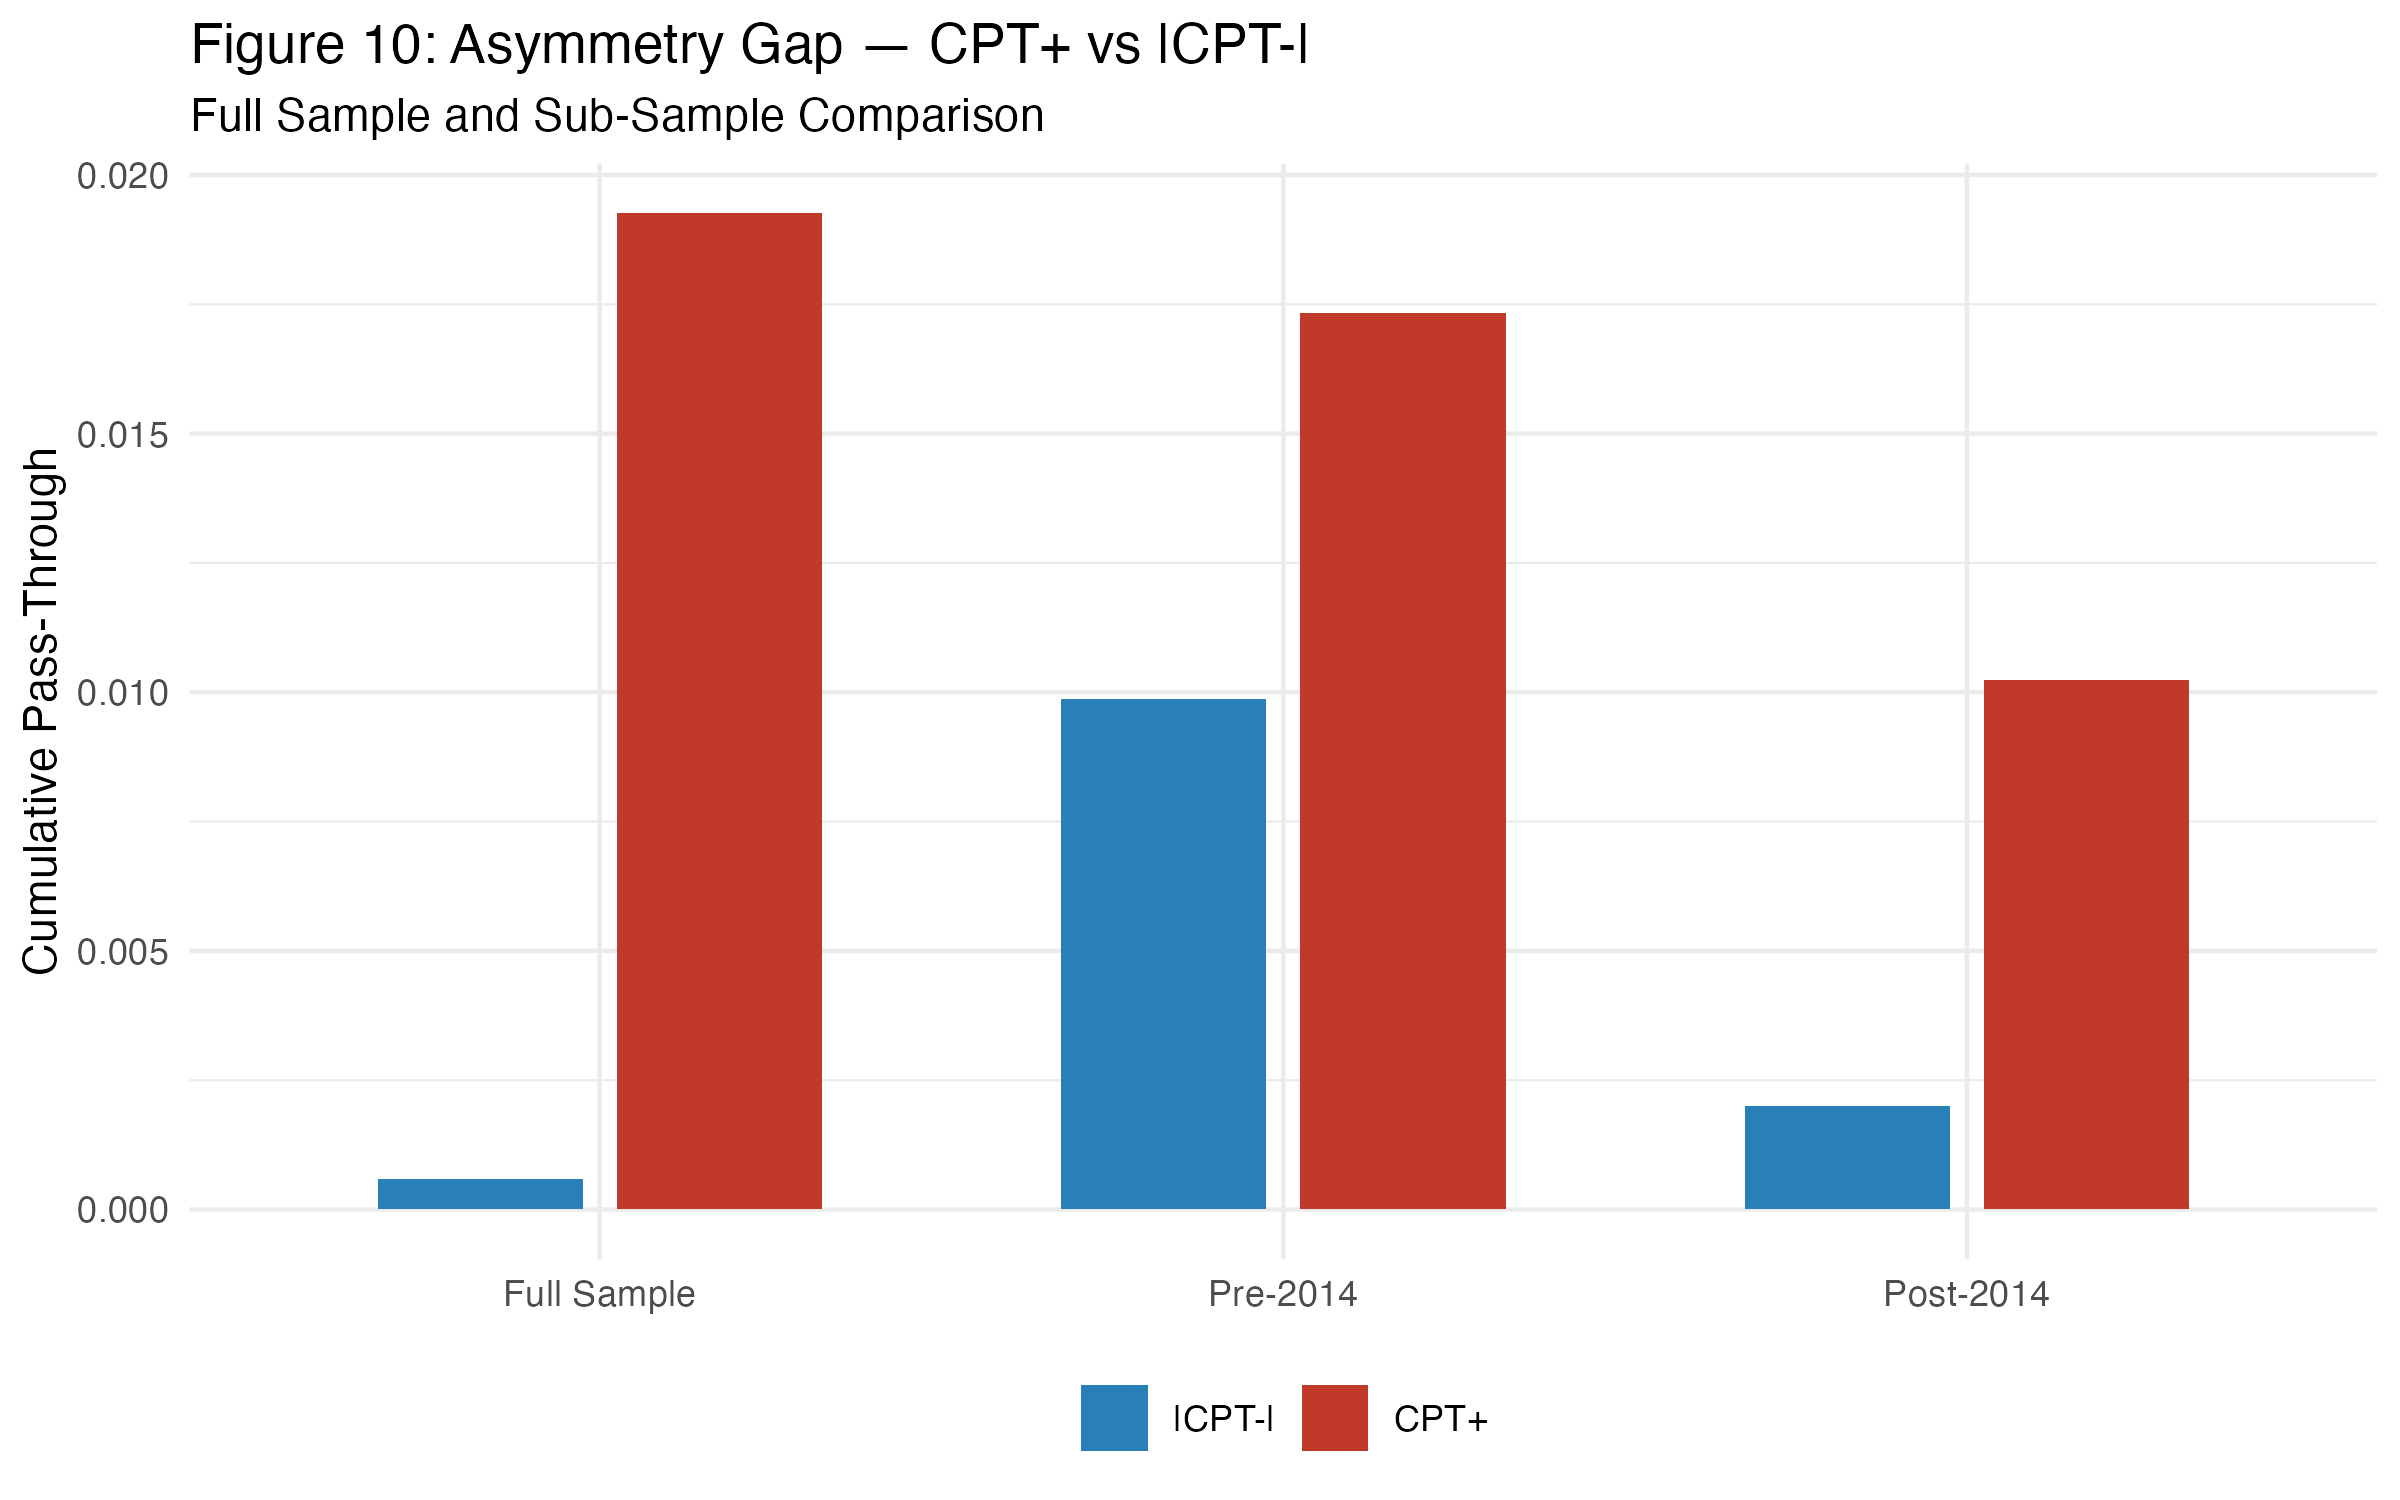
\includegraphics[width=0.78\textwidth]{outputs/figures/fig_10_asymmetry_gap.png}
\caption{Asymmetry gap across full sample and sub-samples}
\label{fig:asymgap}
\end{figure}


% ═══════════════════════════════════════════════════
\section{Summary}
% ═══════════════════════════════════════════════════

\begin{enumerate}[leftmargin=*, noitemsep]

\item The main model is an asymmetric ADL(3,3) with Newey-West HAC inference. Oil lag length is fixed at $q = 3$. AR lag $p = 3$ is selected by AIC.

\item Positive oil shocks have a cumulative pass-through of 0.0213. A 10\% oil price increase raises monthly CPI inflation by about 0.21 percentage points.

\item Negative oil shocks have a cumulative pass-through of 0.0006, which is basically zero.

\item The Wald test for asymmetry does not reject at 5\% ($p = 0.241$). The point estimates are clearly asymmetric, but the statistical evidence is not conclusive for headline CPI.

\item The exchange rate is a significant channel. In the Brent + EXR specification, the exchange rate coefficient is significant at 5\%.

\item The Fuel and Light CPI sub-group gives a significant positive pass-through (CPT$^+ = 0.061$, $p = 0.034$). This is about three times the headline CPI effect.

\item All diagnostic tests pass at 5\%, except heteroskedasticity, which is handled by Newey-West.

\item Results are robust across different lag orders, with and without the COVID dummy, with winsorised shocks, and in rolling windows.

\end{enumerate}

\end{document}
